%%%%%%%% ICML 2024 EXAMPLE LATEX SUBMISSION FILE %%%%%%%%%%%%%%%%%

\documentclass{article}

% Recommended, but optional, packages for figures and better typesetting:
\usepackage{microtype}
\usepackage{graphicx}
\usepackage{subfigure}
\usepackage{booktabs} % for professional tables

% hyperref makes hyperlinks in the resulting PDF.
% If your build breaks (sometimes temporarily if a hyperlink spans a page)
% please comment out the following usepackage line and replace
% \usepackage{icml2024} with \usepackage[nohyperref]{icml2024} above.
\usepackage{hyperref}
\usepackage[normalem]{ulem}

% Attempt to make hyperref and algorithmic work together better:
\newcommand{\theHalgorithm}{\arabic{algorithm}}

% Use the following line for the initial blind version submitted for review:
\usepackage{icml2024}

% If accepted, instead use the following line for the camera-ready submission:
% \usepackage[accepted]{icml2024}

% For theorems and such
\usepackage{amsmath}
\usepackage{amssymb}
\usepackage{mathtools}
\usepackage{amsthm}
\usepackage{bbm}


% if you use cleveref..
\usepackage[capitalize,noabbrev]{cleveref}

%%%%%%%%%%%%%%%%%%%%%%%%%%%%%%%%
% THEOREMS
%%%%%%%%%%%%%%%%%%%%%%%%%%%%%%%%
\theoremstyle{plain}
\newtheorem{theorem}{Theorem}[section]
\newtheorem{proposition}[theorem]{Proposition}
\newtheorem{lemma}[theorem]{Lemma}
\newtheorem{corollary}[theorem]{Corollary}
\theoremstyle{definition}
\newtheorem{definition}[theorem]{Definition}
\newtheorem{assumption}[theorem]{Assumption}
\theoremstyle{remark}
\newtheorem{remark}[theorem]{Remark}

% Todonotes is useful during development; simply uncomment the next line
%    and comment out the line below the next line to turn off comments
%\usepackage[disable,textsize=tiny]{todonotes}
\usepackage[textsize=tiny]{todonotes}


% The \icmltitle you define below is probably too long as a header.
% Therefore, a short form for the running title is supplied here:
\icmltitlerunning{Data-dependent and Oracle Bounds on Forgetting in Continual Learning}




\usepackage{natbib}

\usepackage{times} 
\usepackage{helvet}  
\usepackage{courier}  
\usepackage{url}  
\usepackage{graphicx} 

\usepackage{amssymb}
\usepackage{amsthm}
\usepackage{amsmath}


\usepackage{multirow}
\usepackage{ctable}
\usepackage{color}
\usepackage{natbib}
\usepackage[normalem]{ulem}


\usepackage{hyperref}
\hypersetup{
	colorlinks=true,
	linkcolor=black, % color for table of contents
	citecolor=black, % color for citations
	urlcolor=blue, % color for hyperlinks
	bookmarks=true,
}
\urlstyle{same}

\newcommand{\RM}[1]{{\textcolor{magenta}{#1}}}
\newcommand{\LF}[1]{{\textcolor{blue}{#1}}}
%%%%%%%%%%%%%%%%%%%%%%%%%%%%%%%%%%%%%%%%%%%%%%%%%%%%%%%%%%%%%%%%%%%%%%%%%%%%%%%%%%%%%%%%%%%%%%%%%

\begin{document}

\twocolumn[
\icmltitle{Data-dependent and Oracle Bounds on Forgetting in Continual Learning}
	
% It is OKAY to include author information, even for blind
% submissions: the style file will automatically remove it for you
% unless you've provided the [accepted] option to the icml2024
% package.

% List of affiliations: The first argument should be a (short)
% identifier you will use later to specify author affiliations
% Academic affiliations should list Department, University, City, Region, Country
% Industry affiliations should list Company, City, Region, Country

% You can specify symbols, otherwise they are numbered in order.
% Ideally, you should not use this facility. Affiliations will be numbered
% in order of appearance and this is the preferred way.
\icmlsetsymbol{equal}{*}

\begin{icmlauthorlist}
\icmlauthor{Lior Friedman}{equal,yyy}
\icmlauthor{Ron Meir}{equal,yyy}

\end{icmlauthorlist}

\icmlaffiliation{yyy}{Department of Electrical Engineering, Technion, Haifa, Israel}

\icmlcorrespondingauthor{Lior Friedman}{liorf@campus.technion.ac.il}


% You may provide any keywords that you
% find helpful for describing your paper; these are used to populate
% the "keywords" metadata in the PDF but will not be shown in the document
\icmlkeywords{Machine Learning, ICML}

\vskip 0.3in
]

% this must go after the closing bracket ] following \twocolumn[ ...

% This command actually creates the footnote in the first column
% listing the affiliations and the copyright notice.
% The command takes one argument, which is text to display at the start of the footnote.
% The \icmlEqualContribution command is standard text for equal contribution.
% Remove it (just {}) if you do not need this facility.

%\printAffiliationsAndNotice{}  % leave blank if no need to mention equal contribution
\printAffiliationsAndNotice{\icmlEqualContribution} % otherwise use the standard text.

\begin{abstract}
    In continual learning, knowledge must be preserved and re-used between tasks, maintaining good transfer to future tasks and minimizing forgetting of previously learned ones. While several practical algorithms have been devised for this setting, there have been few theoretical works aiming to quantify and bound the degree of Forgetting in general settings. We provide both data-dependent and oracle upper bounds that apply regardless of model and algorithm choice, as well as bounds for Gibbs posteriors. We derive an algorithm inspired by our bounds and demonstrate empirically that our approach yields improved forward and backward transfer.
\end{abstract}

%\RM{Refer to the theorems in the appendix as theorems or corollaries, depending on their source in the text (currently all are stated as theorems)}\LF{DONE}
\section{Introduction}

Continual learning is a burgeoning machine learning setting where data from different tasks
are presented sequentially to the learner. The usual stated goal of methods in this setting is to adapt the learner to new tasks as they appear while also preserving its performance on previous tasks \cite{de2021continual, hadsell2020embracing,parisi2019continual}.
This performance on previous tasks is called backward transfer, or forgetting, and one of the key challenges in continual learning is avoiding \emph{Catastrophic Forgetting} \cite{goodfellow2014empirical,ramasesh2020anatomy,kirkpatrick2017overcoming}, meaning that performance on previous tasks degrades significantly as the model adapts to new tasks. 

While there have been several empirical methods in the field, there are relatively few theoretical works that explore and attempt to quantify and bound this backward transfer. Some, such as \citet{evron2022catastrophic, lin2023theory} focus on linear models to consider the effect of task order and similarity on forgetting. Others, such as \citet{bennani2020generalisation, doan2021theoretical} utilize the NTK regime to focus on more complex task similarity measures as predictors of forgetting.
Several more general works such as \citet{benavides2022theory} apply notions of VC-dimension to arrive at more general scaling laws and upper bounds on forgetting, but may be difficult to apply for larger models due to the potentially large VC-dimension of models such as deep neural networks \citep{bartlett2019nearly}. %\citet{asanuma2021statistical} explore forgetting in a relatively simple teacher-student setup, and measure task similarity both in input space via distribution comparisons, as well as in parameter space via the cosine distance of weights for the teacher networks.

We note that many of the known results \citep{bennani2020generalisation, evron2022catastrophic,  benavides2022theory} provide upper bound on forgetting for the training data. Our work, however, will focus on bounds on forgetting for test data.

In this work, we will explore upper bounds on forgetting that apply for both general and specific models. We will use the PAC-Bayes \cite{Mcallester, Catoni2004, alquier2021user} %\RM{Add Alquier's review} 
framework to derive and analyze upper bounds on backward transfer, focusing on the Gibbs posterior \citep{casella1992explaining}. We will derive general bounds for the two-task setting, either with no model assumptions or assumptions only on the model for the initial task. We then focus our discussion on oracle bounds for the Gibbs posterior in general, and under specific assumptions of task similarity. We extend these oracle bounds to the general multiple task setting and derive an algorithm inspired by our bounds and compare it to several simple approaches for continual learning\footnote{Code will be made available for the print-ready version.}.

\section{Problem Definition}
%
We consider a finite sequence of tasks $\{1,2,\ldots,T\}\triangleq [T]$, where for each task $k\in[T]$, we are given a batch of data  $S_k\sim \mathcal{D}_k$. 
The sample for a given task $\mathcal{D}$ is defined as $S=\{(x_i,y_i)_{i=1}^m\}$ where $x_i\in \mathcal{X}, y_i\in \mathcal{Y}$.
 A hypothesis $h\in \mathcal{H}$ is a mapping $h:\mathcal{X}\rightarrow \mathcal{Y}$, and is characterized by a loss $\ell(h,z)$.

\begin{definition}
	The expected loss of a given hypothesis $h\in \mathcal{H}$ is defined as $\mathcal{L}(h, \mathcal{D}) \triangleq E_{z\in \mathcal{D}} \ell(h, z)$. The empirical loss of a hypothesis w.r.t.~a sample $S\in \mathcal{D}$ is defined as $\hat{\mathcal{L}}(h, S) \triangleq \frac{1}{m}\sum_{j=1}^{m}\ell(h, z_j)$.
\end{definition}

In this Section, and in Section \ref{sec:oracle-bounds}, we consider only two tasks $\mathcal{D}_s, \mathcal{D}_t$, referring to source and target. Let $Q_s$ be a distribution over the set of hypotheses learned by some algorithm $J_s$ over $S_s\sim \mathcal{D}_s$ and a data-free prior hypothesis distribution $P$, such that $$Q_s=J_s(S_s, P).$$ We then proceed to utilize another algorithm $J_t$ that operates on $S_t\sim \mathcal{D}_t$, making use of $Q_s$, such that 
$$Q_{s:t}=J_t(S_t, Q_s).$$ 
For now, we make no assumptions on $J_s,J_t$ other than their inputs. Of particular note is that $J_t$ has access to information on the previous task only via the prior distribution $Q_s$.

\begin{definition}
	The \emph{backwards transfer loss} of $Q_{s:t}$ on task $\mathcal{D}_s$ is defined as $$\mathrm{BWT}(Q_{s:t}, \mathcal{D}_s) \triangleq \mathbb{E}_{h\sim Q_{s:t}}\left [\mathcal{L}(h, \mathcal{D}_s)\right ]=\mathcal{L}(Q_{s:t}, \mathcal{D}_s).$$
	%
	The \emph{negative transfer} of $Q_{s:t}$ on task $\mathcal{D}_s$ is defined as $$F(Q_{s:t}, \mathcal{D}_s) \triangleq \mathrm{BWT}(Q_{s:t}, \mathcal{D}_s) - \mathbb{E}_{h\sim Q_{s}}\left [\mathcal{L}(h, \mathcal{D}_s)\right ].$$
	%
\end{definition}
Intuitively, the backward transfer $\mathcal{L}(Q_{s:t}, \mathcal{D}_s)$ measures the performance of the updated model on the previous task $\mathcal{D}_s$, and the forgetting $F(Q_{s:t}, \mathcal{D}_s)$ measures how much worse this performance is compared to the loss immediately after learning $S_s\sim\mathcal{D}_s$.

We note that this definition refers to the test forgetting, meaning the model's ability to still generalize well on previously seen domains, rather than measuring the retention of training performance on previous tasks. Due to this definition, simple measures such as memorization of previous training tasks cannot effectively minimize forgetting.
%
\begin{definition}
    The transfer loss of $Q_{s:t}$ on task $\mathcal{D}_t$ is defined as $\mathcal{L}(Q_{s:t}, \mathcal{D}_t)$, and is often referred to as the generalization loss.
\end{definition}

Compared to the backward transfer, the notion of forward transfer (i.e., generalization) is better explored in general, and in the continual learning setting in particular, and several bounds are available \cite{bennani2020generalisation, benavides2022theory}. 
\begin{definition}
    The empirical \emph{Gibbs posterior}, or Gibbs distribution for $Q_s$ with parameter $\lambda$, is defined as 
\begin{equation} \label{defn:gibbs}
\hat Q^\lambda_s(h)=\frac{P(h)e^{-\lambda\hat{\mathcal{L}}(h,S_s)}}{\mathbb{E}_{h\sim P}\left [e^{\lambda\hat{\mathcal{L}}(h,S_s)} \right ]}~ .
\end{equation}
\end{definition}

%=========================================================================
\section{Data-dependent bounds for forgetting}\label{sec:data-dep-bounds}

Throughout the paper, we focus on classification problems.
In order to arrive at an upper bound on the backward transfer, we make use of concentration inequalities, specifically the following specialization of the generic change-of-measure inequality attributed to \citet{donsker1975large}:
% Shui proof actually prove this without the variational lemma, but derivation from the lemma is easy

\begin{lemma} \label{lemma:concentration} \cite{shui2020beyond} Let $\pi$ and $\rho$ be two distributions on a common space $\mathcal{Z}$ such that $\rho$ is absolutely continuous w.\!r.\!t.\! $\pi$. For any $\lambda_t\in \mathbb{R}$ and any measurable function $f:\mathcal{Z}\rightarrow \mathbb{R}$ such that $\mathbb{E}_{z\sim \pi}\left [e^{\lambda_t(f(z)-\mathbb{E}_\pi f(z))} \right ]<\infty$, we have
%
	\begin{equation}
 \begin{split}
	\lambda_t&\left ( \mathbb{E}_{z\sim \rho}\left [f(z) \right ]-\mathbb{E}_{z\sim \pi}\left [f(z) \right ] \right ) \leq \\
 &D_{\mathrm{KL}}(\rho||\pi)+ \log\mathbb{E}_{z\sim \pi}\left [e^{\lambda_t(f(z)-\mathbb{E}_\pi f(z))} \right ],
 \end{split}
	\end{equation}	
	where $D_{\mathrm{KL}}$ is the KL-divergence and equality is achieved for $f(z)=\mathbb{E}_\pi f(z)+\frac{1}{\lambda_t}\log(\frac{d\rho}{d\pi})$.
\end{lemma}

From this lemma, we can arrive at our first result.
%
\begin{theorem} \label{thm:forget-base2}
    For any fixed $S_s,S_t,Q_s,Q_{s:t}$, and $
    \lambda_t>0$, 
    \begin{align} \label{eq:forget-base2}
\mathcal{L}(Q_{s:t}, \mathcal{D}_s) &\leq \hat{\mathcal{L}}(Q_{s:t}, S_t) + \frac{1}{\lambda_t} D_{\mathrm{KL}}(Q_{s:t}||Q_{s})\\
&+\frac{1}{\lambda_t}\log\mathbb{E}_{h\sim Q_{s}}\left [e^{\lambda_t(\mathcal{L}(h,\mathcal{D}_s)-\hat{\mathcal{L}}(h,S_t))} \right ].\nonumber
\end{align}
\end{theorem}
Proof of Theorem \ref{thm:forget-base2} is provided in Appendix \ref{append:proofs}. 
Unlike standard transfer results, the l.h.s.\ depends on the source task $s$ while the r.h.s.\ depends on $t$.

From this point on, we assume that the loss is bounded, though commonly used methods used for proving PAC-Bayes bounds can be applied to extend these results for unbounded Sub-Gaussian or Sub-Gamma losses \citep{alquier2016properties, alquier2021user}.
\begin{assumption}
The loss is bounded, $\ell\in [0, K].$
\end{assumption}
The empirical loss in \eqref{eq:forget-base2} can be removed from the final term leading to the following result.

\begin{corollary}\label{thm:first}
For any fixed $S_s,Q_s,Q_{s:t},\lambda_t>0$, with probability at least $1-\delta/2$ over the choice of $S_t$,
\begin{align}
\mathcal{L}(Q_{s:t}, \mathcal{D}_s) &\leq \hat{\mathcal{L}}(Q_{s:t}, S_t) + \frac{1}{\lambda_t} D_{\mathrm{KL}}(Q_{s:t}||Q_{s})\nonumber\\
&+\frac{1}{2\lambda_t}\log \mathbb{E}_{h\sim Q_{s}}\left [e^{2\lambda_t(\mathcal{L}(h,\mathcal{D}_s)-\mathcal{L}(h,\mathcal{D}_t))}\right ]\nonumber\\ &+\frac{\lambda_t K^2}{4m_t}+\frac{1}{2\lambda_t}\log(2/\delta) .
\end{align}
\end{corollary}

Proof of Corollary \ref{thm:first} is provided in Appendix \ref{append:proofs}. The term $\frac{1}{2\lambda_t}\log \mathbb{E}_{h\sim Q_{s}}\left [e^{2\lambda_t(\mathcal{L}(h,\mathcal{D}_s)-\mathcal{L}(h,\mathcal{D}_t)}\right ]$ measures domain disagreement over $Q_s$, and can be hard to quantify in general. As an informative example, we  consider the special case of the Gibbs distribution.
%
\begin{corollary}
 \label{thm:gibbs-general}
For any $\lambda_t>0$, if \eqref{defn:gibbs} holds, we have with probability at least $1-\delta/2$ over the choice of $S_s,S_t$, for any $Q_{s:t}$, 
%
\begin{align}
\mathcal{L}(Q_{s:t}, \mathcal{D}_s&) \leq \hat{\mathcal{L}}(Q_{s:t}, S_t) + \frac{1}{\lambda_t} D_{\mathrm{KL}}(Q_{s:t}||\hat{Q}_{s}^{2\lambda_t}) \\
&+\frac{\lambda_t K^2}{4m_s}+\frac{\lambda_t K^2}{4m_t}+\frac{1}{\lambda_t}\log(2/\delta)+ \hat{\mathcal{L}}(P, S_s) . \nonumber
\end{align}
\end{corollary}
%
Proof of Corrollary \ref{thm:gibbs-general} is provided in Appendix \ref{append:proofs}. We see that in this setting, the domain disagreement reduces to the loss of the prior $P$ on the first task, alongside having a sufficiently representative sample size for said task.

\section{Oracle bounds for forgetting and transfer}\label{sec:oracle-bounds}

In this section we consider bounds on performance relative to that of an oracle who \emph{knows} the data-distribution, as opposed to the data-dependent bounds established in Section \ref{sec:data-dep-bounds}. Specifically, we consider the Gibbs learner
\begin{equation}\label{eq:Gibbd-dustrib}
\hat{Q}^{\lambda_t}_{s:t}(h)=\frac{Q_s(h)e^{-\lambda_t\mathcal{L}(h,S_t)}}{\mathbb{E}_{h\sim Q_s}\left [e^{-\lambda_t\mathcal{L}(h,S_t)}\right ]}~, 
\end{equation}
where $Q_s$ is arbitrary.
Note that as opposed to \eqref{defn:gibbs}, here the distribution takes into account $S_t$ in addition to $S_s$.

\begin{theorem} \label{thm:oracle-base}
For any $Q_s, S_s, \lambda_t>0$, 
\begin{align} \label{eq:oracle-base}
\mathbb{E}_{S_t\sim \mathcal{D}_t}&\mathcal{L}( \hat{Q}^{\lambda_t}_{s:t},\mathcal{D}_s)\leq \nonumber \\ 
&\inf_{Q_{s:t}}\left \{ \mathcal{L}(Q_{s:t},\mathcal{D}_t) + \frac{1}{\lambda_t}D_{\mathrm{KL}}(Q_{s:t}||Q_{s}) \right \} \\
&+\frac{\lambda_t K^2}{8m_t}+\frac{1}{\lambda_t}\log\mathbb{E}_{h\sim Q_s}\left [e^{\lambda_t\Delta \mathcal{L}(h,s,t)} \right ].\nonumber 
\end{align}
%
where $\Delta \mathcal{L}(h,s,t)\triangleq \mathcal{L}(h,\mathcal{D}_s)-\mathcal{L}(h,\mathcal{D}_t)$.
\end{theorem}
%
Proof of Theorem \ref{thm:oracle-base} is provided in Appendix \ref{append:proofs}. Equation \eqref{eq:oracle-base} contains a \emph{domain disagreement} term, $$\mathrm{Dis}(Q_s,\mathcal{D}_s, \mathcal{D}_t, \lambda_t )\triangleq\frac{1}{\lambda_t}\log\mathbb{E}_{h\sim Q_s}\left [e^{\lambda_t\Delta \mathcal{L}(h,s,t)} \right ].$$

We note that this term may be negative, and that 
$$\mathbb{E}_{h\sim Q_s}\left [\Delta \mathcal{L}(h,s,t) \right ] \leq \mathrm{Dis}(Q_s,\mathcal{D}_s, \mathcal{D}_t, \lambda_t ),$$
as well as,
$$\mathrm{Dis}(Q_s,\mathcal{D}_s, \mathcal{D}_t, \lambda_t )\leq \max_{h}\left [\Delta \mathcal{L}(h,s,t) \right ].$$

Consider a specific setting where the tasks are similar such that 
\begin{equation} \label{eq:assume-similar}
    0\leq \mathrm{Dis}(Q_s,\mathcal{D}_s, \mathcal{D}_t, \lambda_t ) \leq \epsilon_{s,t},
\end{equation}

We can easily arrive at the following Corollary (see full proof in Appendix \ref{append:proofs}).
\begin{corollary}
For any $S_s, \lambda_t>0$, 
    if $Q_s$ obeys \eqref{eq:assume-similar},
    then
    \begin{equation}
\mathbb{E}_{S_s\sim \mathcal{D}_s}\mathbb{E}_{S_t\sim \mathcal{D}_t}F(\hat{Q}^{\lambda_t}_{s:t},\mathcal{D}_t)\leq \frac{\lambda_t K^2}{8m_t} + 2\epsilon_{s,t} .
    \end{equation}
\end{corollary}

\subsection{Oracle bounds with discrepancy terms}

 As we can see from Theorem \ref{thm:oracle-base}, the behavior of $Q_s$ with regard to both tasks can affect the bound quite significantly. 
 While Theorem \ref{thm:oracle-base} demonstrates the importance of $Q_s$, the exact effect of this distribution is unclear. In this section we will discuss several corollaries that provide us with a clearer role for $Q_s$ that defines its desired behavior.
 %As such, we may be interested in other bounds that utilize similar discrepancy terms with regard to $Q_s$.
 The basic oracle inequality theorem we start from is the following (proof in appendix \ref{append:proofs}).
%
\begin{corollary} \label{thm:oracle-logsum}
For any given $S_s\sim \mathcal{D}_s, Q_s, \lambda_t>0$, 
%
\begin{align} \label{eq:oracle-logsum}
\mathbb{E}_{S_t\sim \mathcal{D}_t}&\mathcal{L}( \hat{Q}^{\lambda_t}_{s:t},\mathcal{D}_s)\leq \frac{\lambda_t K^2}{8m_t}\\&+\frac{\mathbb{E}_{h\sim Q_s}\left [e^{\lambda_t\Delta \mathcal{L}(h,s,t)}\mathcal{L}(h,\mathcal{D}_s) \right ]}{\mathbb{E}_{h\sim Q_s}\left [e^{\lambda_t\Delta \mathcal{L}(h,s,t)}\right ]}, \nonumber
\end{align}
\end{corollary}

% In Appendix \ref{append:proofs}, we arrive at a more explicit bound. 

% \begin{corollary}
%  \label{thm:oracle-final}
% For any given $Q_s, \lambda_t>0, S_s\sim \mathcal{D}_s$,  
% %
% \begin{align} \label{eq:oracle-final}
% \mathbb{E}_{S_t\sim \mathcal{D}_t}\mathcal{L}( \hat{Q}^{\lambda_t}_{s:t},&\mathcal{D}_s)\leq \frac{\lambda_t K^2}{8m_t} \nonumber \\
% &+\frac{\sqrt{\mathbb{E}_{Q_s}\left [e^{2\lambda_t\Delta \mathcal{L}(h,s,t)}\right ]}}{\mathbb{E}_{Q_s}\left [e^{\lambda_t\Delta \mathcal{L}(h,s,t)}\right ]}\\
% &\cdot \left (\sqrt{\mathrm{Var}_{Q_s}(\mathcal{L}(h,\mathcal{D}_s))}+\mathcal{L}(Q_s,\mathcal{D}_s)\right )\nonumber
% \end{align}
% \end{corollary}

% This equation gives us three terms that quantify forgetting in terms of $Q_s$.
% \begin{enumerate}
% 	\item The term $$\frac{\sqrt{\mathbb{E}_{Q_s}\left [e^{2\lambda_t\Delta \mathcal{L}(h,s,t)}\right ]}}{\mathbb{E}_{Q_s}\left [e^{\lambda_t\Delta \mathcal{L}(h,s,t)}\right ]}$$ connects the exponential moments of the discrepancies. This term is non-negative, and is upper bounded by $$\max\left \{e^{\lambda_t\max_h\left \{\Delta \mathcal{L}(h,s,t)\right \}},\quad  e^{\lambda_t(\mathcal{L}(Q_s,\mathcal{D}_t)-\mathcal{L}(Q_s,\mathcal{D}_s))}\right \}$$ 
% 	\item The term $\sqrt{\mathrm{Var}_{Q_s}(\mathcal{L}(h,\mathcal{D}_s))}$ is the standard deviation of the expected loss over $Q_s$, and will be low if $Q_s$ is stable in terms of the expected error.
% 	\item The term $\mathcal{L}(Q_s,\mathcal{D}_s)$ is the expected loss of $Q_s$, and will be low if $Q_s$ generalizes well.
% \end{enumerate}

% Unsurprisingly, if $\lambda_t$ is high we arrive at a trivial bound on forgetting, as the Gibbs learner focuses on minimizing the empirical error for $S_t$.

A more explicit bound can be derived from \eqref{eq:oracle-logsum}, see Corollary \ref{corollary:appendix} in the Appendix.
% \begin{corollary}\label{cor:Bhatia}
% For any $\lambda_t>0$,
%
% \begin{align}
% &\mathbb{E}_{S_s\sim \mathcal{D}_s}\mathbb{E}_{S_t\sim \mathcal{D}_t}\mathcal{L}( \hat{Q}^{\lambda_t}_{s:t},\mathcal{D}_s) \leq \frac{\lambda_t K^2}{8m_t} \\
% &+\max_h \left \{ e^{2\lambda_t|\Delta \mathcal{L}(h,s,t)|}\right \}\mathbb{E}_{S_s\sim \mathcal{D}_s}\left [\mathcal{L}(Q_s,\mathcal{D}_s)\right ] .\nonumber 
% \end{align}
% \end{corollary}
%
\subsection{Gibbs posterior bounds}
So far we have focused on oracle bounds for the Gibbs posterior for any prior $Q_s$. A further simplification can be obtained by considering the Gibbs prior \eqref{defn:gibbs},  $Q_s=\hat{Q}^{\lambda_t}_{s}(h).$

We then obtain from our definition of the domain disagreement term that  
\begin{equation*}
\begin{split}
    \mathbb{E}_{S\sim \mathcal{D}_s}&\mathrm{Dis}(\hat{Q}^{\lambda_t}_{s},\mathcal{D}_s, \mathcal{D}_t, \lambda_t )\leq \frac{\lambda_t K^2}{8m_s} -\mathcal{L}(P,\mathcal{D}_t) \\&-\frac{1}{\lambda_t}\mathbb{E}_{S\sim \mathcal{D}_s}\log\mathbb{E}_{h\sim P}\left [e^{-\lambda_t\hat{\mathcal{L}}(h,S)} \right ].
\end{split}
\end{equation*}

Plugging this into \eqref{eq:oracle-base} and using Jensen's inequality, we obtain the following theorem.

\begin{theorem}
For any $\lambda_t>0$, if $Q_s$ obeys \eqref{defn:gibbs}, 
%
\begin{equation}
\begin{split}
&\mathbb{E}_{S_s\sim \mathcal{D}_s}\mathbb{E}_{S_t\sim \mathcal{D}_t}\mathcal{L}( \hat{Q}^{\lambda_t}_{s:t},\mathcal{D}_s)\leq \mathbb{E}_{S_s\sim \mathcal{D}_s}\mathcal{L}(\hat{Q}^{\lambda_t}_s,\mathcal{D}_t)\\&+\frac{\lambda_t K^2}{8m_t}+\frac{\lambda_t K^2}{8m_s}+\mathcal{L}(P,\mathcal{D}_s)-\mathcal{L}(P,\mathcal{D}_t).
\end{split}
\end{equation}
\end{theorem}

This provides us with a more practical prior $\hat{Q}^{\lambda_t}_s$ at the cost of additional approximation error $\lambda_t K^2/8m_s$.
If $m_s,m_t\rightarrow \infty$\footnote{In this case, $\hat{Q}^\lambda_s=Q^\lambda_s, \hat{Q}^{\lambda_t}_{s:t}=Q^{\lambda_t}_{s:t}$}, we get an interesting bound involving generalization and forgetting,
%
\begin{equation*}
\begin{split}
\mathbb{E}_{S_s\sim \mathcal{D}_s}\mathbb{E}_{S_t\sim \mathcal{D}_t}\mathcal{L}( \hat{Q}^{\lambda_t}_{s:t},\mathcal{D}_s)&-\mathbb{E}_{S_s\sim \mathcal{D}_s}\mathcal{L}(\hat{Q}^{\lambda_t}_s,\mathcal{D}_t)\\&\leq \mathcal{L}(P,\mathcal{D}_s)-\mathcal{L}(P,\mathcal{D}_t)
\end{split}
\end{equation*}

We note that the right-hand-side is data-free and describes the general loss landscapes of both tasks with respect to the prior $P$. If both tasks come from the same distribution, for example, this implies that forgetting is upper bounded by the forward transfer (for Gibbs measures).
This suggests that any problem with high forgetting for the Gibbs measure would also have poor forward transfer and a problem with good forward transfer will also have low forgetting. 

\subsection{Learning Gibbs posteriors without forgetting}

So far, we have derived oracle bounds that offer useful insights on the backward transfer for the Gibbs posterior. We would also like to examine whether stronger assumptions can offer bounds with improved or vanishing forgetting.
Considering \eqref{eq:oracle-base}, we can consider the situation where $Q_s$ is given by \eqref{defn:gibbs} from a different angle.

\begin{theorem}
For any $\lambda_t>0$, if \eqref{defn:gibbs} holds, 
%
\begin{equation} 
\begin{split}
\mathbb{E}_{S_s\sim \mathcal{D}_s}&\mathbb{E}_{S_t\sim \mathcal{D}_t}\mathcal{L}( \hat{Q}^{\lambda_t}_{s:t},\mathcal{D}_s)\leq \frac{\lambda_t K^2}{8m_t}+\frac{\lambda_t K^2}{8m_s}\\&+\mathcal{L}(P,\mathcal{D}_s)+\mathcal{L}(P,\mathcal{D}_t) \\&+\frac{1}{\lambda_t}\log\mathbb{E}_{h\sim P}\left [e^{-\lambda_t\mathcal{L}(h,\mathcal{D}_t)} \right ] .
\end{split}
\end{equation}
\end{theorem}

Compare this to forward transfer (proved in Appendix \ref{append:proofs}).
\begin{theorem}
For any $\lambda_t>0$, if \eqref{defn:gibbs} holds, 
%
\begin{equation} 
\begin{split}
\mathbb{E}_{S_s\sim \mathcal{D}_s}\mathbb{E}_{S_t\sim \mathcal{D}_t}&\mathcal{L}( \hat{Q}^{\lambda_t}_{s:t},\mathcal{D}_t)\leq \frac{\lambda_t K^2}{8m_t}+\frac{\lambda_t K^2}{8m_s}\\&+\mathcal{L}(P,\mathcal{D}_s)+\mathcal{L}(P,\mathcal{D}_t) \\&+\frac{1}{\lambda_t}\log\mathbb{E}_{h\sim P}\left [e^{-\lambda_t\mathcal{L}(h,\mathcal{D}_s)} \right ] .
\end{split}
\end{equation}
\end{theorem}

We can see that in both cases, the loss is bounded by functions of sample size originating from the deviations of sample from its mean (e.g. Hoeffding's inequality), and the loss of the data-free prior, which serves as a limit if no additional information on the tasks is available.

One such source of additional information is the \emph{covariance} of the losses, which we use as a measure of task similarity. 
%
$$
\mathrm{cov}_{\lambda_t}(P,s,t)\triangleq \mathrm{cov}_{h\sim P}\left (e^{-\lambda_t\hat{\mathcal{L}}(h,S_s)}, e^{-\lambda_t\hat{\mathcal{L}}(h,S_t)}\right ).
$$
%
% \begin{equation*} 
% \begin{split}
% &\mathbb{E}_{h\sim P}\left [e^{-\lambda_t\mathcal{L}(h,\mathcal{D}_t)-\lambda_t\mathcal{L}(h,\mathcal{D}_s)}\right ]\\&=\mathbb{E}_{h\sim P}\left [e^{-\lambda_t\mathcal{L}(h,\mathcal{D}_t)}\right ] \mathbb{E}_{h\sim P}\left [e^{-\lambda_t\mathcal{L}(h,\mathcal{D}_s)}\right ]\\&+\mathrm{cov}_{h\sim P}\left (e^{-\lambda_t\mathcal{L}(h,\mathcal{D}_s)}, e^{-\lambda_t\mathcal{L}(h,\mathcal{D}_t)}\right )
% \end{split}
% \end{equation*}
%
We note that this covariance term is bounded in $[-1, 1]$. From this decomposition, we have:
%
\begin{corollary} \label{thm:cov-2task}
For any $\lambda>0$, if \eqref{defn:gibbs} holds, and $\mathrm{cov}_{\lambda_t}(P,s,t)\geq 0$,      
\begin{align} 
\mathbb{E}_{S_s\sim \mathcal{D}_s}\mathbb{E}_{S_t\sim \mathcal{D}_t}\mathcal{L}( \hat{Q}^{\lambda_t}_{s:t},\mathcal{D}_s)&\leq \frac{\lambda_t K^2}{8m_s}+\mathcal{L}(P,\mathcal{D}_s)\\
%
\mathbb{E}_{S_s\sim \mathcal{D}_s}\mathbb{E}_{S_t\sim \mathcal{D}_t}\mathcal{L}( \hat{Q}^{\lambda_t}_{s:t},\mathcal{D}_t)&\leq \frac{\lambda_t K^2}{8m_t}+\mathcal{L}(P,\mathcal{D}_t) 
\end{align}
\end{corollary}

We can further improve upon this bound given a tighter bound on the covariance.
%
\begin{corollary}
\label{thm:cov-2task-highcov}
For any $\lambda>0$, if \eqref{defn:gibbs} holds, and $\mathrm{cov}_{\lambda_t}(P,s,t)\geq e^{-c}$,    
%
\begin{equation} 
\mathbb{E}_{S_s\sim \mathcal{D}_s}\mathbb{E}_{S_t\sim \mathcal{D}_t}\mathcal{L}( \hat{Q}^{\lambda_t}_{s:t},\mathcal{D}_s)\leq \frac{\lambda_t K^2}{8m_s}+\frac{c}{\lambda_t}
\end{equation}
%
\begin{equation} 
\mathbb{E}_{S_s\sim \mathcal{D}_s}\mathbb{E}_{S_t\sim \mathcal{D}_t}\mathcal{L}( \hat{Q}^{\lambda_t}_{s:t},\mathcal{D}_t)\leq \frac{\lambda_t K^2}{8m_t}+\frac{c}{\lambda_t} 
\end{equation}
\end{corollary}

Both Corollaries \ref{thm:cov-2task} and \ref{thm:cov-2task-highcov} are specific cases of more general Theorems that apply for any finite number of tasks. These bounds will be presented in the following subsection.

We note that if the covariance is negative we can suffer at worst a term proportional to $K$, thereby making the bound vacuous in the worst case. This is unsurprising, as it means that the hypotheses that perform well on the source task perform poorly on the target and vice versa, which makes learning to generalize without forgetting impossible.

We note that the phenomenon of self-forgetting seen in the NTK regime in \citet{karakida2021learning} can also be seen in our bounds: if $m_s$ is small we can get forgetting even if the target task is the same (high covariance), and learning the same task again with new data may be worse than using all of the data as a single training set.

\subsection{Extension to $T$ tasks}

Suppose we are given a set of tasks $\{1,2,\ldots, T\} = [T]$, appearing sequentially.
We would like to minimize the average backward transfer after all tasks, $$\frac{1}{T}\sum_{i=1}^T
\mathbb{E}_{S_i}\mathcal{L}(\hat{Q}^{\lambda_T}_{1:T}, \mathcal{D}_i),$$ where $Q_{1:i}$ is the posterior after $i$ sequential tasks. In general, this definition does not assume anything about the construction of the posterior, other than the fact that we have no access to samples from future (unseen) tasks while learning each specific posterior $Q_{1:i}$. $\hat{Q}^{\lambda_T}_{1:T}$ is the empirical Gibbs posterior for sample $S_T$ and prior $Q_{1:T-1}$.

To do so, we focus on bounding the individual losses for each task.
Using the same change of measure inequality as in Theorem \ref{thm:forget-base2}, we can derive the following general bound on forgetting. 

\begin{theorem} $\mathrm{(Forgetting)}$
For any $\lambda_T>0$, for any $S_T\sim \mathcal{D}_T$ and $i\in [T-1]$,
%
\begin{align} \label{eq:forget-base-T}
\begin{split}
&\mathcal{L}(Q_{1:T}, \mathcal{D}_i) \leq \hat{\mathcal{L}}(Q_{1:T}, S_T)\\ &+ \frac{1}{\lambda_T} D_{\mathrm{KL}}(Q_{1:T}||Q_{1:T-1})
\\&+\frac{1}{\lambda_T}\log\mathbb{E}_{h\sim Q_{1:T-1}}\left [e^{\lambda_T(\mathcal{L}(h,\mathcal{D}_i)-\hat{\mathcal{L}}(h,S_T))} \right ]
\end{split}
\end{align}
\end{theorem}

Starting from \eqref{eq:forget-base-T}, we show in appendix \ref{append:proofs} that if all of the priors are empirical Gibbs distributions, namely
$$\forall i\in\{2,\ldots,T\}, ~~\hat{Q}^{\lambda_i}_{1:i}(h)\propto \hat{Q}^{\lambda_{i-1}}_{1:i-1}(h)e^{-\lambda_i\hat{\mathcal{L}}(h,S_i)}$$ 
where $\hat{Q}^{\lambda_1}_{1:1}(h)\propto P(h)e^{-\lambda_1\hat{\mathcal{L}}(h,S_1)}$, we have the following.

\begin{theorem} $\mathrm{(Forgetting)}$ \label{thm:forgetting-extended}
For any $\lambda_T>0$, assuming all $Q_{1:j}$ are empirical Gibbs posteriors, and that
 $\mathrm{cov}_{P}(i, [T])\geq 0$,
for any sample of training sets $S_{j}\sim \mathcal{D}_j$, then $\forall i\in[T-1]$
%
\begin{align} \label{eq:forgetting-extended}
\begin{split}
\mathbb{E}_{S_i}\mathcal{L}(\hat{Q}^{\lambda_T}_{1:T}, \mathcal{D}_i) &\leq \frac{\lambda_T K^2}{8m_i}+\mathcal{L}(P,\mathcal{D}_i).
\end{split}
\end{align}
\end{theorem}
%
As the extension to the covariance for two tasks, we have a similar notion of covariance 
$$\mathrm{cov}_{P}(i, [T])\triangleq\mathrm{cov}_{P}(e^{-\lambda_T\hat{\mathcal{L}}(h,S_i)}, e^{-\sum_{j=1,j\neq i}^{T}\lambda_j\hat{\mathcal{L}}(h,S_j)}).$$
%
As far as forward transfer, we can apply a similar analysis (for standard change-of-measure). 
%
\begin{theorem} $\mathrm{(Transfer)}$ 
For any $\lambda_T>0$, if all $Q_{1:j}$ are empirical Gibbs posteriors,
and $\mathrm{cov}_{P}(T, [T])\geq 0$,
for any sample of training sets $S_{j< T}\sim \mathcal{D}_j$,
%
\begin{align} 
\begin{split}
\mathbb{E}_{S_T}\mathcal{L}(\hat{Q}^{\lambda_T}_{1:T}, \mathcal{D}_T) &\leq \frac{\lambda_T K^2}{8m_T}+\mathcal{L}(P,\mathcal{D}_T) .
\end{split}
\end{align}
\end{theorem}
%
Theorem \ref{thm:forgetting-extended} is somewhat surprising, as it implies a sufficient condition for learning without forgetting that, for each individual task, does not become worse with the number of tasks and has no direct dependence on task order or on the length of time a task has not been seen. While the r.h.s.~in \eqref{eq:forgetting-extended} contains a constant term $\mathcal{L}(P,\mathcal{D}_i)$, we note that this term does not depend on the number of total tasks $T$ or on $i$. We also note that the negative transfer $F(\hat{Q}^{\lambda_T}_{1:T}, \mathcal{D}_i)$ may be negative. We show in Corollary \ref{thm:oracle-T-highcov} that a stronger condition on the covariance even leads to vanishing forgetting.

This lack of dependence on task order can be attributed to the nature of the empirical Gibbs distribution that applies a combination of exponential weights on the initial distribution $P$. The final weight of any given hypothesis $h$ therefore does not depend on the order of tasks but rather only on $P(h)$ and its empirical performance on each task.

The fact that this bound does not become worse with the number of tasks is a result of the assumption on the non-negative covariance: we assume that hypotheses that perform well on task $i$ tend to perform well on all other tasks, and thus the exponential weighting scheme does not significantly reduce their probability in the final distribution. 

% We note that in general we also know (even if the covariance is not negative) \RM{Explain why this is important} that
% \begin{align} 
% \begin{split}
% \mathbb{E}_{S_T}\mathcal{L}(\hat{Q}^{\lambda_T}_{1:T}, \mathcal{D}_T) &\leq \frac{\lambda_T K^2}{8m_T}+\mathcal{L}(\hat{Q}^{\lambda_{T-1}}_{1:T-1},\mathcal{D}_T) .
% \end{split}
% \end{align}

If we make stronger assumptions on this covariance, we can arrive at a potentially tighter bound.

\begin{corollary}
\label{thm:oracle-T-highcov}
    Under the same conditions as Theorem \ref{thm:forgetting-extended}, if we additionally have
%
\begin{align*} 
\begin{split}
&\mathrm{cov}_{P}(i, [T])
  \geq e^{-c}-\mathbb{E}_{h\sim P}\left [e^{-\lambda_T\hat{\mathcal{L}}(h,S_i)} \right ] \geq 0,
\end{split}
\end{align*}
%
we have (for any sample of training sets $S_{j}\sim \mathcal{D}_j$):
%
\begin{align*} 
\begin{split}
\forall i\in[T-1]:
\mathbb{E}_{S_i}\mathcal{L}(\hat{Q}^{\lambda_T}_{1:T}, \mathcal{D}_i) &\leq \frac{\lambda_T K^2}{8m_i}+\frac{c}{\lambda_T}.
\end{split}
\end{align*}
\end{corollary}

This implies that if, for example, 
$\mathrm{cov}_{P}(i, [T])
 \geq e^{-c/T}$,
 we have increasingly reduced average forgetting (assuming $\lambda_T\leq \min_i m_i$) as more tasks are seen, since  
\begin{align*} 
\begin{split}
\frac{1}{T}\sum_{i=1}^T
\mathbb{E}_{S_i}\mathcal{L}(\hat{Q}^{\lambda_T}_{1:T}, \mathcal{D}_i) &\leq \frac{\lambda_T K^2}{8T}\sum_{i=1}^T\frac{1}{m_i}+\frac{c}{T\lambda_T}.
\end{split}
\end{align*}

%=========================================================================
\section{Empirical study}

In this section we demonstrate our approach on both synthetic and real-world data sets. We study five classes of task environments, with very different types of shifts between tasks.

While Theorem \ref{thm:forgetting-extended} provides an oracle bound, we can use it and its task similarity measure as an inspiration for a general continual learning algorithm, described in Algorithm \ref{alg:naive-forgetting}. Intuitively, we see that if $C_{i,j}$ is negative, there is inherent interference between the new task $i$ and previous tasks, meaning that removing it is preferable (line $10$). For tasks with positive $C_{i,j}$, our bounds show that higher covariance implies lower risk of forgetting, and so we increase the relative weight for such tasks by increasing $\lambda$ proportionally to $C_{i,j}$ (line $12$).

\begin{algorithm}[H]
	\caption{CL-FORC: Continual Learning without FORgetting via Covariance conditions}
	\label{alg:naive-forgetting}
	\small
	\begin{algorithmic}[1]
		\STATE {\bfseries Continual-learn} ($S_1,\ldots, S_T$, $P$)
		\STATE Choose algorithmic parameters $\lambda_1,\ldots, \lambda_T$
		\STATE Let $\hat{Q}_{1:0}(h) \triangleq P(h)$
		\FOR {each task $i$ from $1$ to $T$} 
		\STATE Store $S_i$
            \STATE Save posterior $\hat{Q}_{1:i}(h)\propto \hat{Q}_{1:i-1}(h)e^{-\lambda_i \hat{\mathcal{L}}(h,S_i)}$
		\FOR {each previous task from $1$ to $i-1$} 
		\STATE Let $C_{i,j}=\textrm{Cov}_{\hat{Q}_{1:j-1}}(e^{-\lambda_j \hat{\mathcal{L}}(h,S_j)}, e^{-\sum_{j< k\leq i}\lambda_k \hat{\mathcal{L}}(h,S_k)})$
            \IF {$C_{i,j}<0$} 
                \STATE Remove task $j$, unlearn it by $\hat{Q}_{1:i}(h)\propto \hat{Q}_{1:i}(h)e^{\lambda_j \hat{\mathcal{L}}(h,S_j)}$
                \ELSIF{$C_{i,j}\geq 0$} 
                    \STATE $\lambda_j \leftarrow (2-C_{i,j})\lambda_j$ 
                \ENDIF
		\ENDFOR 
		\ENDFOR
		\STATE {\bfseries Return} $\hat{Q}_{1:T}$
	\end{algorithmic}
\end{algorithm}

Since Algorithm \ref{alg:naive-forgetting} may be difficult to implement in practice due the difficulties in modeling the Gibbs posterior, we consider a more practical version of it, given in Algorithm \ref{alg:empirical-forgetting}. This version assumes Gaussian distributions, performs gradient descent, and uses the average KL-divergence in line $6$ rather than computing the full posterior.  

\begin{algorithm}[H]
	\caption{Practical implementation of Algorithm \ref{alg:naive-forgetting}}
	\label{alg:empirical-forgetting}
	\small
	\begin{algorithmic}[1]
 \STATE {\bfseries Continual-learn}($S_1,\ldots, S_T$, $P=\mathcal{N}(\mu, \Sigma)$)
		\STATE Choose algorithmic parameters $\lambda_1 = \lambda_2 = \cdots = \lambda_T=\lambda$
		\STATE Let $\hat{Q}_{1:0}(h) \triangleq P(h)$
		\FOR {each task $i$ from $1$ to $T$} 
		\STATE Store $S_i$
            \STATE Learn posterior $\hat{Q}_{1:i}$ via SGD on $\hat{\mathcal{L}}(\hat{Q}_{1:i}, S_i)+\sum_{j=1}^{i-1}\frac{1}{\lambda_j}D_{KL}(\hat{Q}_{1:i}||\hat{Q}_{1:j})$
		\FOR {each previous task $j$ from $1$ to $i-1$} 
		\STATE Let $C_{i,j}=\textrm{Cov}_{\hat{Q}_{1:j-1}}(e^{-\lambda_j \hat{\mathcal{L}}(h,S_j)}, e^{-\sum_{j< k\leq i}\lambda_k \hat{\mathcal{L}}(h,S_k)})$
            \IF {$C_{i,j}<0$} 
                \STATE Set $\lambda_j=\infty$ \COMMENT{Remove task $j$}
                \ELSIF{$C_{i,j}\ge 0$} 
                    \STATE $\lambda_j \leftarrow (2-C_{i,j})\lambda_j$ 
                \ENDIF
		\ENDFOR 
		\ENDFOR
		\STATE  {\bfseries Return} $\hat{Q}_{1:T}$
	\end{algorithmic}
\end{algorithm}

We also note that using the Pearson correlation instead of the covariance in line 8 leads to more stable results.

\subsection{Experimental settings}

In order to measure the performance of Algorithm \ref{alg:empirical-forgetting}, we must define the relevant metrics we wish to measure. These are the backwards transfer $\sum_{i=1}^{T}\mathcal{L}(\hat{Q}_{1:T}, \mathcal{D}_i)$ (measured via a separate test set per task), the average forward transfer $\frac{1}{T}\sum_{i=1}^{T}\mathcal{L}(\hat{Q}_{1:i}, \mathcal{D}_i)$ (measured via a separate test set per task), and finally the forward transfer for the recent few tasks, e.g., $\frac{1}{5}\sum_{i=T-5}^{T}\mathcal{L}(\hat{Q}_{1:i}, \mathcal{D}_i)$ 

We compare Algorithm \ref{alg:empirical-forgetting} to several baseline methods for continual learning. All of these methods use Algorithm \ref{alg:empirical-forgetting}, without lines $7\rightarrow 12$, reflecting the task-covariances, and replace the objective in line $6$ as follows:
\begin{itemize}
    \item SGD: $\hat{\mathcal{L}}(\hat{Q}_{1:i}, S_i)$.
    \item PAC-Bayes (PB):  $\hat{\mathcal{L}}(\hat{Q}_{1:i}, S_i)+\frac{1}{\lambda}D_{\mathrm{KL}}(\hat{Q}_{1:i}||P)$.
    \item Averaged PB: Use the same objective as Algorithm \ref{alg:empirical-forgetting}, but  $\lambda_i$ parameters are static and equal.
\end{itemize}

In the following experiments, we use fully connected neural networks with a separate linear head per task to facilitate measuring the forgetting without re-training linear heads. We use Adam \citep{KingmaB14} for optimization. The full list of hyper-parameters is listed in \ref{append:hyperparam}. 

\subsection{Simple tasks: $2d$ Gaussian data}\label{sec:Gaussian-data}

We begin by examining several setups of binary classification tasks in $\mathbb{R}^2$. All tasks draw samples from a $2$-dimensional Gaussian distribution $p(x) = \mathcal{N}(x;0,I_2)$, and $y=\mathrm{sgn}(a^\top x)$. We use several setups for task ordering in order to better examine the covariance term $C_{i,j}$ and its effect under different setups. Specifically, we consider the following settings:
(1) Similar tasks: linear separators for all tasks are within $10^\circ$ of some reference angle.
    (2) Distractors: like ``Similar tasks" but $20\%$  of tasks have reversed labels.
    (3) Gradual shift: tasks change angle gradually in a set direction, with each consecutive task being within $10^\circ$ of the last one.
    (4) Orthogonal tasks: two sets of similar tasks with a $90^\circ$ angle between the separators of both task sets. Tasks alternate between both types.
    (5) Orthogonal shift: Similar to ``Orthogonal tasks", but the first half of tasks are of the first type and the second half corresponds to the second type.

We used a total of $T=100$ tasks in this domain in order to observe general trends.
We note that these problems differ significantly in task order and overall behavior, and are aimed to provide a diverse set of challenges to our algorithm. In addition, we should not expect a single algorithm to perform optimally across all settings, as known empirical methods based on regularization would perform poorly on orthogonal tasks whereas replay-based and architecture-based methods would have issues with gradual shift. We expect that in real-world settings, prior knowledge can be used to suggest specific algorithms.

In particular, the settings of Distractors, Gradual shift and Orthogonal shifts are constructed such that forgetting may be desirable. A recent paper by \citet{kumar2023continual} discusses continual learning as a computationally constrained optimization problem and argues that forgetting non-recurring information is not ``catastrophic", especially given changing environments. Of our constructed settings, these three are those where not all previous knowledge is beneficial.

% \begin{figure*}[ht!]
% %\vskip 0.2in
% \centering
% 	\subfigure[Similar tasks.]{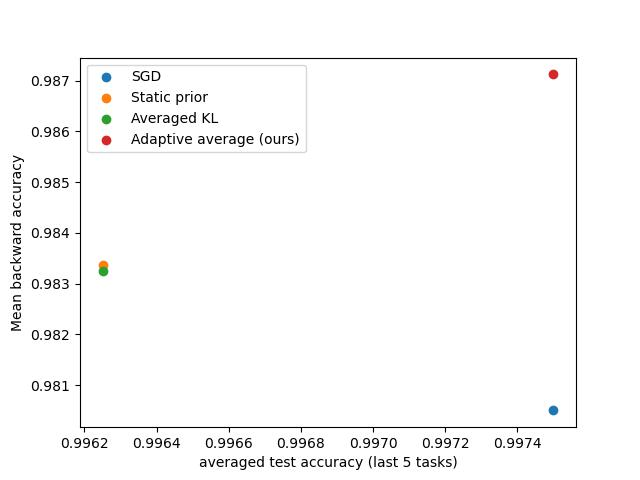
\includegraphics[width=0.19\textwidth]{tradeoffs_last5_positive_correlation}}	
%  \subfigure[Distractors.]{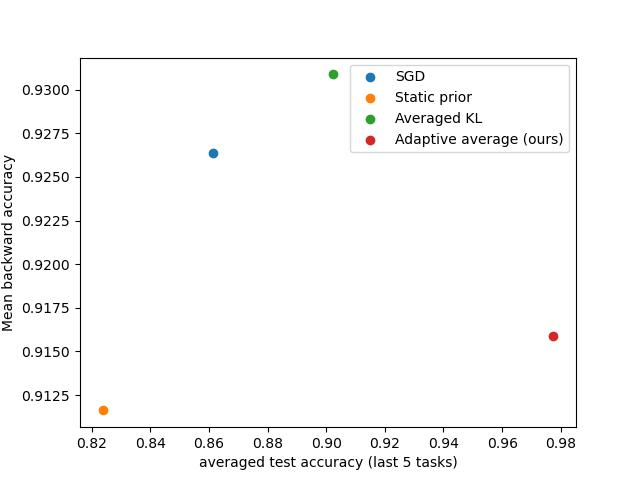
\includegraphics[width=0.19\textwidth]{tradeoffs_last5_distractors}}
%  \subfigure[Gradual shift.]{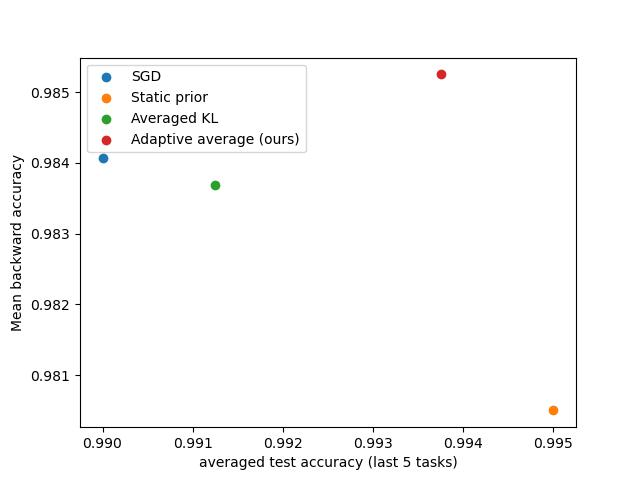
\includegraphics[width=0.19\textwidth]{tradeoffs_last5_gradual_shift}}
%  \subfigure[Orthogonal tasks.]{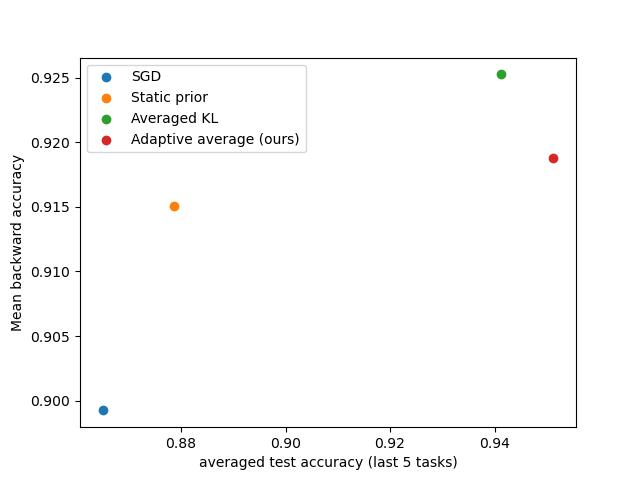
\includegraphics[width=0.19\textwidth]{tradeoffs_last5_orthogonal_alternating}}
%  \subfigure[Orthogonal shift.]{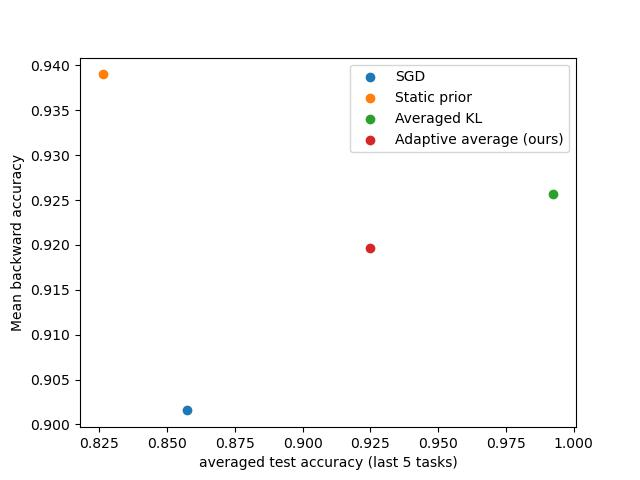
\includegraphics[width=0.19\textwidth]{tradeoffs_last5_orthogonal_shift}}

% \caption{Average test accuracy for last $5$ tasks vs average backward transfer for a variety of task settings for synthetic Gaussian data.}
% \label{2d-test-error}
% %\vskip -0.2in
% \end{figure*}

\begin{table}[t]
\caption{Metrics for $2d$ continual tasks. All test metrics are in averaged accuracy percentage over the relevant models and test sets. Backward transfer is averaged accuracy over all test sets.}
%\RM{What is the std for these experiments?}
\label{2d-full-table}
\vskip 0.15in
\begin{center}
\begin{small}
\begin{sc}
\begin{tabular}{lccc}
\toprule
Method & Back. acc. & Test acc. & last $5$ acc. \\
\midrule
Similar tasks & & & \\
\midrule
SGD    & $98$ & $99$ & $\mathbf{99.7}$ \\
PB & $98.3$ & $99.3$ & $99.6$\\
Averaged    & $98.3$ & $99.3$ & $99.6$ \\
CL-FORC    & $\mathbf{98.7}$& $\mathbf{99.5}$ & $\mathbf{99.7}$        \\

\\Distractors & & & \\
\midrule
SGD    & $92.6$ & $\mathbf{94.2}$ & $86.1$ \\
PB & $91.1$ & $92.3$ & $82.4$\\
Averaged    & $\mathbf{93.1}$ & $93.6$ & $90.3$ \\
CL-FORC    & $91.6$& $92.7$ & $\mathbf{97.7}$        \\

\\ Gradual shift & & & \\
\midrule
SGD    & $93$ & $94$ & $93.4$ \\
PB & $91$ & $92.5$ & $83.2$\\
Averaged    & $\mathbf{94.1}$ & $\mathbf{94.5}$ & $84.8$ \\
CL-FORC    & $92.6$& $94.4$ & $\mathbf{94.6}$        \\

\\ Orth. tasks & & & \\
\midrule
SGD    & $89.9$ & $90.9$ & $86.5$ \\
PB & $91.5$ & $93$ & $87.9$\\
Averaged    & $\mathbf{92.5}$ & $\mathbf{93.4}$ & $94.1$ \\
CL-FORC    & $91.9$& $93.2$ & $\mathbf{95.1}$        \\

\\ Orth. shift & & & \\
\midrule
SGD    & $90.2$ & $91$ & $85.8$ \\
PB & $\mathbf{93.9}$ & $\mathbf{94.4}$ & $82.6$\\
Averaged    & $92.6$ & $93.8$ & $\mathbf{99.2}$ \\
CL-FORC    & $92$& $93.6$ & $92.5$        \\

\bottomrule
\end{tabular}
\end{sc}
\end{small}
\end{center}
\vskip -0.1in
\end{table}

Table \ref{2d-full-table} describes the forward and backward transfer for the $2d$ tasks. We can see that Algorithm \ref{alg:empirical-forgetting} tends to provide good forward transfer for both the the last few tasks as well as the overall forward transfer. We can also see that despite the fact that this algorithm is inspired by a bound focusing on forgetting, Algorithm \ref{alg:empirical-forgetting} tends to have higher overall forgetting compared to using all previous models with equal relative weight. 
As noted in the previous paragraph, forgetting may be desirable in some circumstances, and we see that our approach tends to have worse backward transfer in such settings.

One possible explanation for the higher than expected forgetting can be obtained by looking at the practical effect of the weighting scheme created by Algorithm \ref{alg:empirical-forgetting} on model weights: weights for uncorrelated tasks are halved on each subsequent task, and maintaining high relative weight (and thus high importance) requires very high covariance between tasks. For the ``distractors" task set, for example, our approach actively forgets distracting tasks by assigning them low weight (since the covariance is negative), and old tasks are slowly forgotten due to the fact that the covariance is not always highly positive.

This behavior demonstrated by the ``distractors" task set can also be seen to a lesser extent in the other task sets for the $2d$ setting, and suggests that the covariance measure used in Algorithm \ref{alg:empirical-forgetting} is a useful (if perhaps conservative) method to determine whether a task should be actively forgotten.

\subsection{Vision tasks: CIFAR-$10$}

In this section, we examine Algorithm \ref{alg:empirical-forgetting} on a more realistic problem domain, namely sequential binary classification tasks constructed from the CIFAR-$10$ \citep{krizhevsky2009learning} dataset. We used $T=200$ tasks in order to explore long term changes in overall performance.

We consider two specific continual problems. In the first, from the ``domain-incremental continual learning" setup \citep{de2021continual}, tasks differ by the samples used for each. Specifically, we generate a binary classification problem by taking samples from the ``automobile" vs ``truck" classes.   In the second, we use a similar scheme to ``orthogonal shift" from the $2d$ setting. A set of tasks from the ``automobile" vs ``truck" domain, followed by a set of tasks from the ``cat" vs ``dog".

\begin{figure*}[ht]
\vskip 0.2in
\centering
	\subfigure[Averaged test accuracy over time.]{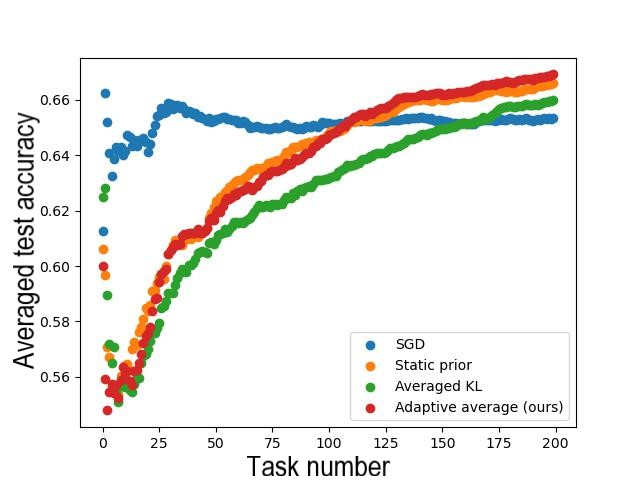
\includegraphics[width=0.32\textwidth]{test_errors_cifar10_static}}
 \subfigure[Summed backward accuracy over time.]{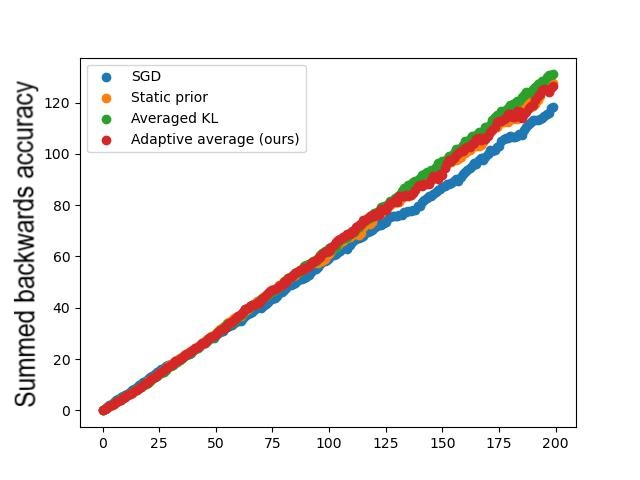
\includegraphics[width=0.32\textwidth]{test_backwards_cifar10_static}}

\caption{Metrics over time (task count) for the domain-incremental setting for CIFAR-$10$. Higher is better. }
\label{cifar-static}
\vskip -0.2in
\end{figure*}

\begin{figure*}[ht!]
\vskip 0.2in
\centering
	\subfigure[Averaged test accuracy over time.]{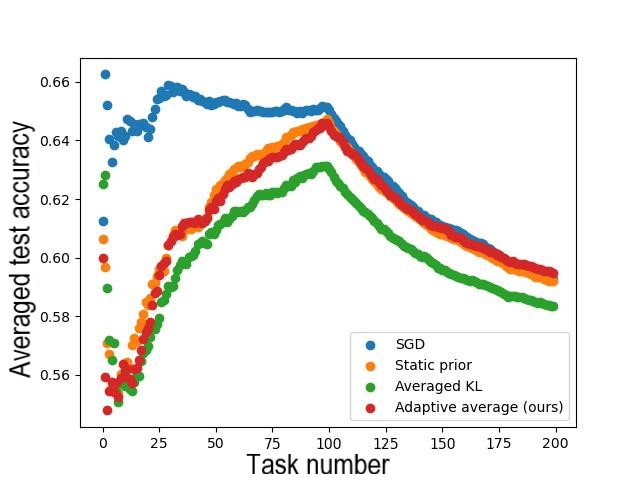
\includegraphics[width=0.32\textwidth]{test_errors_cifar10_shift}}
 \subfigure[Summed backward accuracy over time.]{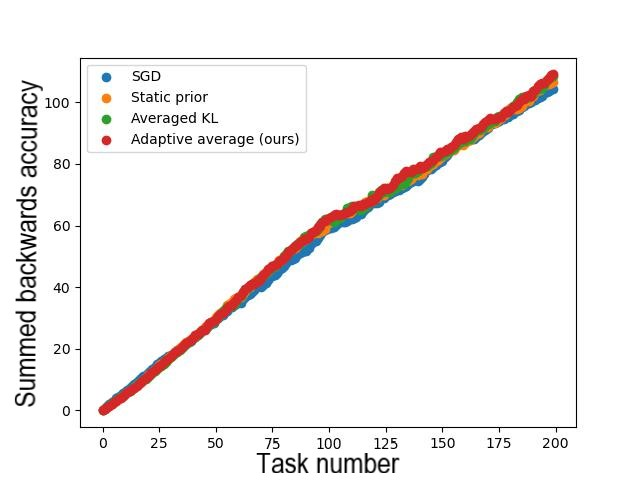
\includegraphics[width=0.32\textwidth]{test_backwards_cifar10_shift}}


\caption{Metrics over time (task count) for the shifting domain setting for CIFAR-$10$. Higher is better. The shift occurs at $T=100$.}
\label{cifar-shift}
\vskip -0.2in
\end{figure*}

\begin{table}[t]
\caption{Metrics for CIFAR-$10$ continual tasks. All test metrics are in averaged accuracy percentage over the relevant models and test sets. Backward transfer is averaged accuracy over all test sets.}
\label{cifar-full-table}
\vskip 0.15in
\begin{center}
\begin{small}
\begin{sc}
\begin{tabular}{lccc}
\toprule
Method & Back. acc. & Test acc. & last $5$ acc. \\
\midrule
$1$ domain & & & \\
\midrule
SGD    & $118.4$ & $65.3$ & $66.1$ \\
PB & $127.8$ & $66.6$ & $\mathbf{70.9}$\\
Averaged    & $\mathbf{131}$ & $66$ & $69.8$ \\
CL-FORC    & $126.3$& $\mathbf{66.9}$ & $70.6$        \\

\\ Shifting & & & \\
\midrule
SGD    & $104.4$ & $59.3$ & $52.2$ \\
PB & $106.6$ & $59.1$ & $53.5$\\
Averaged    & $108.6$ & $58.4$ & $\mathbf{55.1}$ \\
CL-FORC   & $\mathbf{109.5}$& $\mathbf{59.5}$ & $54.8$        \\
\bottomrule
\end{tabular}
\end{sc}
\end{small}
\end{center}
\vskip -0.1in
\end{table}

Figure \ref{cifar-static} shows the gradual change in test accuracy and backward transfer. We can see that all regularized methods have some initial warm-up time before they begin to offer significant advantages over simply learning the tasks in sequence. We can also see that the significant improvement in test forgetting coincides (at least for the data-free approach and ours) with said improvement in forward transfer. Combined with the reported test accuracies for the last $5$ tasks (Table \ref{cifar-full-table}), this suggests that for the domain-incremental setting, backward transfer and forward transfer are strongly linked, as one is indicative of the other.

Figure \ref{cifar-shift} details the shifting domain setting. The clear increase in forgetting combined with a notable drop in test accuracy immediately after the domain shift may be indicative of issues related to network plasticity and the ``stability-plasticity" dilemma \citep{mirzadeh2020understanding} that is commonly associated with continual learning models based on gradient optimization. We note that all regularized approaches tended to slowly recover from this issue.

\section{Conclusions and future work}

In this work, we derived several upper bounds on the test forgetting for both general model classes and for the Gibbs posterior, based on the changes of measure approach.
These upper bounds are data-dependent, potentially offering tighter bounds if improved prior models for the task are available, or if tasks are structured such that their loss landscapes are similar. In particular, we focused on oracle bounds for Gibbs posteriors that offered tight bounds on forgetting if task losses are highly positively correlated, thus making the knowledge accumulation process highly effective for all tasks.

Based on our theoretical bounds, we constructed an algorithm for continual learning with potentially low forgetting that retains and forgets tasks based on the correlation of their loss landscapes. We examined this approach on several simple task constructions as well as a more complex vision task. In our experiments we noted a relation between forward and backward transfer, especially for mostly static settings such as the domain-incremental continual learning problem. As noted by several previous theoretical works and practical examinations (see Introduction), task order and similarity can greatly influence both forgetting and generalization. While this empirical demonstration is not the main focus of our paper, it suggests that using the covariance measure as a metric for task similarity merits further exploration.

Several interesting directions for future research on general models exist. One relevant extension involves using known literature from Transfer Learning \citep{zhuang2020comprehensive} to allow for bounds where loss landscapes are less similar, as well as better quantifying the effects of this similarity on backward transfer.
In a somewhat similar vein, it may be useful to derive general bounds that more explicitly consider task order and similarity measures, perhaps using recent advances in PAC-Bayes bounds for Super-martingales \cite{haddouche2023pac}.
Finally, we can consider more commonly known extensions to PAC-Bayes bounds such as unbounded losses or data-dependent bounds \citep{rivasplata2020pac}.

\section*{Impact statement}
This paper presents work whose goal is to advance the field of Machine Learning. There are many potential societal consequences of our work, none which we feel must be specifically highlighted here.




%We hope that a better theoretical understanding of backward transfer and forgetting, as explored in this work as well as several previous works, can improve our capability to create methods that only forget the irrelevant and effectively utilize beneficial knowledge.

% Acknowledgements should only appear in the accepted version.
%\section*{Acknowledgements}

\clearpage
\bibliographystyle{plainnat}
\bibliography{library}

%%%%%%%%%%%%%%%%%%%%%%%%%%%%%%%%%%%%%%%%%%%%%%%%%%%%%%%%%%%%%%%%%%%%%%%%%%%%%%%
%%%%%%%%%%%%%%%%%%%%%%%%%%%%%%%%%%%%%%%%%%%%%%%%%%%%%%%%%%%%%%%%%%%%%%%%%%%%%%%
% APPENDIX
%%%%%%%%%%%%%%%%%%%%%%%%%%%%%%%%%%%%%%%%%%%%%%%%%%%%%%%%%%%%%%%%%%%%%%%%%%%%%%%
%%%%%%%%%%%%%%%%%%%%%%%%%%%%%%%%%%%%%%%%%%%%%%%%%%%%%%%%%%%%%%%%%%%%%%%%%%%%%%%
\newpage
\appendix
\onecolumn

\section{Appendix - proofs} \label{append:proofs}

\begin{theorem} Restatement of Theorem \ref{thm:forget-base2}:
     For any fixed $S_s,S_t,Q_s,Q_{s:t}$, for any $
    \lambda_t>0$,
    \begin{align} 
\begin{split}
\mathcal{L}(Q_{s:t}, \mathcal{D}_s) &\leq \hat{\mathcal{L}}(Q_{s:t}, S_t) + \frac{1}{\lambda_t} D_{\mathrm{KL}}(Q_{s:t}||Q_{s})\\
&+\frac{1}{\lambda_t}\log\mathbb{E}_{h\sim Q_{s}}\left [e^{\lambda_t(\mathcal{L}(h,\mathcal{D}_s)-\hat{\mathcal{L}}(h,S_t))} \right ]
\end{split}
\end{align}
\end{theorem}

\begin{proof}
    Starting from Lemma \ref{lemma:concentration}, we can choose $f(z)=\mathcal{L}(z,\mathcal{D}_s)-\hat{\mathcal{L}}(z,S_t)$, giving us

\begin{align*}
\begin{split}
\lambda_t\mathbb{E}_{h\sim Q_{s:t}}\left [\mathcal{L}(h,\mathcal{D}_s)-\hat{\mathcal{L}}(h,S_t) \right ] - \lambda_t\mathbb{E}_{h\sim Q_{s}}\left [\mathcal{L}(h,\mathcal{D}_s)-\hat{\mathcal{L}}(h,S_t) \right ] \\
\leq D_{\mathrm{KL}}(Q_{s:t}||Q_{s})+\log\mathbb{E}_{h\sim Q_{s}}\left [e^{\lambda_t(\mathcal{L}(h,\mathcal{D}_s)-\hat{\mathcal{L}}(h,S_t))}e^{-\lambda_t(\mathcal{L}(Q_s,\mathcal{D}_s)-\hat{\mathcal{L}}(Q_s,S_t))} \right ]
\end{split}
\end{align*}

Extracting terms that do not depend on $h$ from the expectation, we get

\begin{align} \label{eq:forget-base}
\begin{split}
F(Q_{s:t},\mathcal{D}_s) &\leq \hat{\mathcal{L}}(Q_{s:t}, S_t) - \mathcal{L}(Q_{s}, D_s) + \frac{1}{\lambda_t} D_{\mathrm{KL}}(Q_{s:t}||Q_{s})\\
&+\frac{1}{\lambda_t}\log\mathbb{E}_{h\sim Q_{s}}\left [e^{\lambda_t(\mathcal{L}(h,\mathcal{D}_s)-\hat{\mathcal{L}}(h,S_t))} \right ]
\end{split}
\end{align}

\end{proof}

%%%%%%%%%%%%%%%%%%%%%%%%%%%%%%%%%%%%%%
\begin{lemma} \label{lemma:hoeffding-concentration}
	Let $l:Z\times H\rightarrow[0,K]$ be a measurable function. Let $\pi\in\mathcal{M}(H)$ be a distribution over $H$ that is independent w.r.t. $Z$. Let $S\in Z^m$ be an i.\! i.\! d.\! sample. With probability at least $1-\delta$ over the choice of $S$,
%	
	$$\log \mathbb{E}_{h\sim \pi}\left [e^{t(\frac{1}{m}\sum_i l(z_i,h)-\mathbb{E}_{z}l(z,h))}\right ]\leq \frac{t^2K^2}{8m}+\log{1/ \delta}$$
\end{lemma}

\begin{proof} 
	Using Markov's inequality, we know that 
	$$\textrm{Pr}\left (\mathbb{E}_{h\sim \pi}\left [e^{t(\frac{1}{m}\sum_i l(z_i,h)-\mathbb{E}_{z}l(z,h))}\right ]<\frac{1}{\delta}\mathbb{E}_{S\sim Z^m}\mathbb{E}_{h\sim \pi}\left [e^{t(\frac{1}{m}\sum_i l(z_i,h)-\mathbb{E}_{z}l(z,h))}\right ] \right ) \geq 1-\delta$$
	
	Applying Fubini's theorem (both distributions are independent), we can re-order the expectations
	
	$$\textrm{Pr}\left (\mathbb{E}_{h\sim \pi}\left [e^{t(\frac{1}{m}\sum_i l(z_i,h)-\mathbb{E}_{z}l(z,h))}\right ]<\frac{1}{\delta}\mathbb{E}_{h\sim \pi}\mathbb{E}_{S\sim Z^m}\left [e^{t(\frac{1}{m}\sum_i l(z_i,h)-\mathbb{E}_{z}l(z,h))}\right ] \right ) \geq 1-\delta$$
	
	Since $S$ is drawn i.\! i.\! d.\! and $l$ is bounded, we can apply Hoeffding's lemma to each example, giving us
	
	$$\textrm{Pr}\left (\mathbb{E}_{h\sim \pi}\left [e^{t(\frac{1}{m}\sum_i l(z_i,h)-\mathbb{E}_{z}l(z,h))}\right ]<\frac{1}{\delta}\mathbb{E}_{h\sim \pi}\left [e^{\frac{t^2K^2}{8m}}\right ] \right ) \geq 1-\delta$$
	
	$$\textrm{Pr}\left (\log\mathbb{E}_{h\sim \pi}\left [e^{t(\frac{1}{m}\sum_i l(z_i,h)-\mathbb{E}_{z}l(z,h))}\right ]<\log\frac{1}{\delta}e^{\frac{t^2K^2}{8m}} \right ) \geq 1-\delta$$
	
	and so we have 
	
	$$\textrm{Pr}\left (\log\mathbb{E}_{h\sim \pi}\left [e^{t(\frac{1}{m}\sum_i l(z_i,h)-\mathbb{E}_{z}l(z,h))}\right ]<\log\frac{1}{\delta}+\frac{t^2K^2}{8m} \right ) \geq 1-\delta$$
	
\end{proof}

%%%%%%%%%%%%%%%%%%%%%%%%%%%%%%%%%%%%%%%
%proof for thm:first

\begin{corollary} Restatement of Corollary \ref{thm:first}:
If $\ell\in [0,K]$, for any fixed $S_s,Q_s,Q_{s:t},\lambda_t>0$, with probability at least $1-\delta/2$ over the choice of $S_t$,
\begin{align}
\begin{split}
\mathcal{L}(Q_{s:t}, \mathcal{D}_s) &\leq \hat{\mathcal{L}}(Q_{s:t}, S_t) + \frac{1}{\lambda_t} D_{\mathrm{KL}}(Q_{s:t}||Q_{s})\\
&+\frac{1}{2\lambda_t}\log \mathbb{E}_{h\sim Q_{s}}\left [e^{2\lambda_t(\mathcal{L}(h,\mathcal{D}_s)-\mathcal{L}(h,\mathcal{D}_t))}\right ]\\ &+\frac{\lambda_t K^2}{4m_t}+\frac{1}{2\lambda_t}\log(2/\delta)
\end{split}
\end{align}
\end{corollary}

\begin{proof}
    Starting from \eqref{eq:forget-base}, we note that
    $$\log\mathbb{E}_{h\sim Q_{s}}\left [e^{\lambda_t(\mathcal{L}(h,\mathcal{D}_s)-\hat{\mathcal{L}}(h,S_t))} \right ] = \log\mathbb{E}_{h\sim Q_{s}}\left [e^{\lambda_t(\mathcal{L}(h,\mathcal{D}_s)-\mathcal{L}(h,\mathcal{D}_t)+\mathcal{L}(h,\mathcal{D}_t)-\hat{\mathcal{L}}(h,S_t))} \right ].$$

    This gives us 
$$\log\mathbb{E}_{h\sim Q_{s}}\left [e^{\lambda_t(\mathcal{L}(h,\mathcal{D}_s)-\hat{\mathcal{L}}(h,S_t))} \right ] = \log\mathbb{E}_{h\sim Q_{s}}\left [e^{\lambda_t(\mathcal{L}(h,\mathcal{D}_s)-\mathcal{L}(h,\mathcal{D}_t))}e^{\lambda_t(\mathcal{L}(h,\mathcal{D}_t)-\hat{\mathcal{L}}(h,S_t))} \right ]$$
$$\triangleq \log\mathbb{E}_{Q_{s}}\left [e^{\lambda_t\Delta\mathcal{L}(h,\mathcal{D}_s, \mathcal{D}_t)}e^{\lambda_t\Delta\hat{\mathcal{L}}(h,\mathcal{D}_t, S_t)} \right ].$$

Using the Cauchy-Shwartz inequality $$\mathbb{E}_{X}\left [f_1(X)f_2(X)\right ]^2\leq \mathbb{E}_{X}\left [f_1(X)^2\right ]\mathbb{E}_{X}\left [f_2(X)^2\right ],$$
as well as the fact that both exponent terms are non-negative, we have

\begin{align} \label{eq:cs-diff}
\begin{split}
\log\mathbb{E}_{Q_{s}}\left [e^{\lambda_t\Delta\mathcal{L}(h,\mathcal{D}_s, \mathcal{D}_t)}e^{\lambda_t\Delta\hat{\mathcal{L}}(h,\mathcal{D}_t, S_t)} \right ]\leq \frac{1}{2}\log\mathbb{E}_{Q_{s}}\left [e^{2\lambda_t\Delta\mathcal{L}(h,\mathcal{D}_s, \mathcal{D}_t)}\right ]\mathbb{E}_{Q_{s}}\left [e^{2\lambda_t\Delta\hat{\mathcal{L}}(h,\mathcal{D}_t, S_t)} \right ].
\end{split}
\end{align}

If $\ell\in [0,K]$, we can use Lemma \ref{lemma:hoeffding-concentration} and \eqref{eq:cs-diff} and get with probability at least $1-\delta/2$ over the choice of $S_t$

$$\log\mathbb{E}_{h\sim Q_{s}}\left [e^{\lambda_t(\mathcal{L}(h,\mathcal{D}_s)-\hat{\mathcal{L}}(h,S_t))} \right ]\leq \frac{1}{2}\log\mathbb{E}_{Q_{s}}\left [e^{2\lambda_t\Delta\mathcal{L}(h,\mathcal{D}_s, \mathcal{D}_t)}\right ]+\frac{\lambda_t^2K^2}{4m_t}+\log(2/\delta)$$

\end{proof}

%%%%%%%%%%%%%%%%%%%%%%%%%%%%%%%%%%%%%%%%%%%
% proof for gibbs general

\begin{corollary} Restatement of Corollary \ref{thm:gibbs-general}:
For any $\lambda_t>0$, if $$Q_s(h)=\frac{P(h)e^{-2\lambda_t\hat{\mathcal{L}}(h,S_s)}}{\mathbb{E}_{h\sim P}\left [e^{-2\lambda_t\hat{\mathcal{L}}(h,S_s)} \right ]}$$ and the loss is bounded $\ell\in[0,K]$, 
we have with probability at least $1-\delta/2$ over the choice of $S_s,S_t$, for any $Q_{s:t}$, 
%
\begin{align}
\begin{split}
\mathcal{L}(Q_{s:t}, \mathcal{D}_s) &\leq \hat{\mathcal{L}}(Q_{s:t}, S_t) + \frac{1}{\lambda_t} D_{\mathrm{KL}}(Q_{s:t}||Q_{s})\\
&+\frac{\lambda_t K^2}{4m_s}+\frac{\lambda_t K^2}{4m_t}+\frac{1}{\lambda_t}\log(2/\delta)+ \hat{\mathcal{L}}(P, S_s)
\end{split}
\end{align}
\end{corollary}

\begin{proof}
    Starting from Corollary \ref{thm:first}, we note that
    $$\frac{1}{2\lambda_t}\log \mathbb{E}_{h\sim Q_{s}}\left [e^{2\lambda_t(\mathcal{L}(h,\mathcal{D}_s)-\mathcal{L}(h,\mathcal{D}_t))}\right ]=\frac{1}{2\lambda_t}\log \int \frac{1}{\mathbb{E}_{h\sim P}\left [e^{-2\lambda_t\hat{\mathcal{L}}(h,S_s)} \right ]}P(h)e^{2\lambda_t(\mathcal{L}(h,\mathcal{D}_s)-\hat{\mathcal{L}}(h,S_s)-\mathcal{L}(h,\mathcal{D}_t))}dh$$
    $$=\frac{1}{2\lambda_t}\log \int \frac{\mathbb{E}_{h\sim P} e^{-2\lambda_t\mathcal{L}(h,\mathcal{D}_t)}}{\mathbb{E}_{h\sim P} e^{-2\lambda_t\hat{\mathcal{L}}(h,S_s)}  }\frac{P(h)e^{-2\lambda_t\mathcal{L}(h,\mathcal{D}_t)}}{\mathbb{E}_{h\sim P} e^{-2\lambda_t\mathcal{L}(h,\mathcal{D}_t)}}e^{2\lambda_t(\mathcal{L}(h,\mathcal{D}_s)-\hat{\mathcal{L}}(h,S_s))}dh$$
    $$=\frac{1}{2\lambda_t}\log\frac{\mathbb{E}_{h\sim P} e^{-2\lambda_t\mathcal{L}(h,\mathcal{D}_t)}}{\mathbb{E}_{h\sim P} e^{-2\lambda_t\hat{\mathcal{L}}(h,S_s)}  }+\frac{1}{2\lambda_t}\log\mathbb{E}_{h\sim Q^{*}_t}\left [e^{2\lambda_t(\mathcal{L}(h,\mathcal{D}_s)-\hat{\mathcal{L}}(h,S_s))}\right ]$$

    Using Lemma \ref{lemma:hoeffding-concentration} again gives us with probability at least $1-\delta/2$ over the choice of $S_s$

$$\frac{1}{2\lambda_t}\log \mathbb{E}_{h\sim Q^{*}_t}\left [e^{2\lambda_t(\mathcal{L}(h,\mathcal{D}_s)-\mathcal{L}(h,\mathcal{D}_t))}\right ] \leq \frac{\lambda_t K^2}{4m_s}+\frac{1}{2\lambda_t}\log(2/\delta)$$

Putting it all together with a union bound, if $Q_s(h)=\frac{P(h)e^{-2\lambda_t\hat{\mathcal{L}}(h,S_s)}}{\mathbb{E}_{h\sim P}\left [e^{-2\lambda_t\hat{\mathcal{L}}(h,S_s)} \right ]}$ and the loss is bounded $\ell\in[0,K]$, we have with probability at least $1-\delta/2$ over the choice of $S_s,S_t$,

\begin{align}
\begin{split}
\mathcal{L}(Q_{s:t}, \mathcal{D}_s) &\leq \hat{\mathcal{L}}(Q_{s:t}, S_t) + \frac{1}{\lambda_t} D_{\mathrm{KL}}(Q_{s:t}||Q_{s})
+\frac{\lambda_t K^2}{4m_s}+\frac{\lambda_t K^2}{4m_t}+\frac{1}{\lambda_t}\log(2/\delta)+\frac{1}{2\lambda_t}\log\frac{\mathbb{E}_{h\sim P} e^{-2\lambda_t\mathcal{L}(h,\mathcal{D}_t)}}{\mathbb{E}_{h\sim P} e^{-2\lambda_t\hat{\mathcal{L}}(h,S_s)}  }
\end{split}
\end{align}

We can further simplify this expression 

\begin{align*}
\begin{split}
\mathcal{L}(Q_{s:t}, \mathcal{D}_s) &\leq \hat{\mathcal{L}}(Q_{s:t}, S_t)+ \frac{1}{\lambda_t} D_{\mathrm{KL}}(Q_{s:t}||Q_{s})
+\frac{\lambda_t K^2}{4m_s}+\frac{\lambda_t K^2}{4m_t}+\frac{1}{\lambda_t}\log(2/\delta)\\&+\frac{1}{2\lambda_t}\log\mathbb{E}_{h\sim P} e^{-2\lambda_t\mathcal{L}(h,\mathcal{D}_t)}-\frac{1}{2\lambda_t}\log\mathbb{E}_{h\sim P} e^{-2\lambda_t\hat{\mathcal{L}}(h,S_s)}   \\
& \leq \hat{\mathcal{L}}(Q_{s:t}, S_t)+ \frac{1}{\lambda_t} D_{\mathrm{KL}}(Q_{s:t}||Q_{s})
+\frac{\lambda_t K^2}{4m_s}+\frac{\lambda_t K^2}{4m_t}+\frac{1}{\lambda_t}\log(2/\delta)+0+\frac{1}{2\lambda_t}\mathbb{E}_{h\sim P} 2\lambda_t\hat{\mathcal{L}}(h,S_s) \\
& \leq \hat{\mathcal{L}}(Q_{s:t}, S_t) + \frac{1}{\lambda_t} D_{\mathrm{KL}}(Q_{s:t}||Q_{s})
+\frac{\lambda_t K^2}{4m_s}+\frac{\lambda_t K^2}{4m_t}+\frac{1}{\lambda_t}\log(2/\delta)+ \hat{\mathcal{L}}(P, S_s)
\end{split}
\end{align*}

\end{proof}

%%%%%%%%%%%%%%%%%%%%%%%%%%%%%%%%%%%%%%%%%%%%%%

%proof for oracle:base

\begin{theorem} Restatement of Theorem \ref{thm:oracle-base}:
For any $Q_s, S_s, \lambda_t>0$, if $\ell\in [0,K]$, 
\begin{equation} 
\begin{split}
\mathbb{E}_{S_t\sim \mathcal{D}_t}&\mathcal{L}( \hat{Q}^{\lambda_t}_{s:t},\mathcal{D}_s)\leq\\ &\inf_{Q_{s:t}}\left \{ \mathcal{L}(Q_{s:t},\mathcal{D}_t) + \frac{1}{\lambda_t}D_{\mathrm{KL}}(Q_{s:t}||Q_{s}) \right \} \\
&+\frac{\lambda_t K^2}{8m_t}+\frac{1}{\lambda_t}\log\mathbb{E}_{h\sim Q_s}\left [e^{\lambda_t(\mathcal{L}(h,\mathcal{D}_s)-\mathcal{L}(h,\mathcal{D}_t))} \right ]
\end{split}
\end{equation}
\end{theorem}

\begin{proof}
Starting from Lemma \ref{lemma:concentration}, we know that 

$$\mathbb{E}_{z\sim \rho}\left [f(z) \right ]\leq \mathbb{E}_{z\sim \pi}\left [f(z) \right ]+ \frac{1}{\lambda_t}D_{\mathrm{KL}}(\rho||\pi)+ \frac{1}{\lambda_t}\log\mathbb{E}_{z\sim \pi}\left [e^{\lambda_t(f(z)-\mathbb{E}_\pi f(z))} \right ]$$

In particular, for $\hat{\rho}_\lambda(z)\propto \pi(z) e^{-\lambda_t f(z) }$, this is an equality (from \citeauthor{donsker1975large}'s [\citeyear{donsker1975large}] variational lemma).
From this, we know that

\begin{equation}
\mathbb{E}_{z\sim \hat{\rho}_\lambda}\left [f(z) \right ]= \mathbb{E}_{z\sim \pi}\left [f(z) \right ]+ \frac{1}{\lambda_t}D_{\mathrm{KL}}(\hat{\rho}_\lambda||\pi)+ \frac{1}{\lambda_t}\log\mathbb{E}_{z\sim \pi}\left [e^{\lambda_t(f(z)-\mathbb{E}_\pi f(z))} \right ]
\end{equation}

If we pick $f(z)=\mathcal{L}(z,\mathcal{D}_s)-\hat{\mathcal{L}}(z,S_t)$ as before, we get

$$\mathbb{E}_{z\sim \hat{\rho}_\lambda}\left [\mathcal{L}(z,\mathcal{D}_s) \right ]= \mathbb{E}_{z\sim \pi}\left [f(z) \right ]+\mathbb{E}_{z\sim \hat{\rho}_\lambda}\left [\hat{\mathcal{L}}(z,S_t) \right ]+ \frac{1}{\lambda_t}D_{\mathrm{KL}}(\hat{\rho}_\lambda||\pi)+ \frac{1}{\lambda_t}\log\mathbb{E}_{z\sim \pi}\left [e^{\lambda_t(f(z)-\mathbb{E}_\pi f(z))} \right ]$$

And as such,
$$F( \hat{\rho}_\lambda,\mathcal{D}_s)\leq \inf_{\rho}\left \{ \hat{\mathcal{L}}(\rho,S_t) + \frac{1}{\lambda_t}D_{\mathrm{KL}}(\rho||\pi)  \right \}-\mathcal{L}(\pi,D_s)+\frac{1}{\lambda_t}\log\mathbb{E}_{z\sim \pi}\left [e^{\lambda_t(\mathcal{L}(z,\mathcal{D}_s)-\hat{\mathcal{L}}(z,S_t))} \right ],$$

or using our previous terminology with $\hat{Q}^{\lambda_t}_{s:t}(h)\propto Q_s(h)e^{-\lambda_t\hat{\mathcal{L}}(h,S_t)}$, 

$$\mathcal{L}( \hat{Q}^{\lambda_t}_{s:t},\mathcal{D}_s)\leq \inf_{Q_{s:t}}\left \{ \hat{\mathcal{L}}(Q_{s:t},S_t) + \frac{1}{\lambda_t}D_{\mathrm{KL}}(Q_{s:t}||Q_{s}) \right \}+\frac{1}{\lambda_t}\log\mathbb{E}_{h\sim Q_s}\left [e^{\lambda_t(\mathcal{L}(h,\mathcal{D}_s)-\hat{\mathcal{L}}(h,S_t))} \right ]$$

If we take an expectation on $S_t$, we get

$$\mathbb{E}_{S_t\sim \mathcal{D}_t}\mathcal{L}( \hat{Q}^{\lambda_t}_{s:t},\mathcal{D}_s)\leq \mathbb{E}_{S_t\sim \mathcal{D}_t}\inf_{Q_{s:t}}\left \{ \hat{\mathcal{L}}(Q_{s:t},S_t) + \frac{1}{\lambda_t}D_{\mathrm{KL}}(Q_{s:t}||Q_{s}) \right \}+\frac{1}{\lambda_t}\mathbb{E}_{S_t\sim \mathcal{D}_t}\log\mathbb{E}_{h\sim Q_s}\left [e^{\lambda_t(\mathcal{L}(h,\mathcal{D}_s)-\hat{\mathcal{L}}(h,S_t))} \right ]$$

This gives us the following oracle inequality (in expectation):

$$\mathbb{E}_{S_t\sim \mathcal{D}_t}\mathcal{L}( \hat{Q}^{\lambda_t}_{s:t},\mathcal{D}_s)\leq \inf_{Q_{s:t}}\left \{ \mathcal{L}(Q_{s:t},\mathcal{D}_t) + \frac{1}{\lambda_t}D_{\mathrm{KL}}(Q_{s:t}||Q_{s}) \right \}+\frac{1}{\lambda_t}\log\mathbb{E}_{h\sim Q_s}\mathbb{E}_{S_t\sim \mathcal{D}_t}\left [e^{\lambda_t(\mathcal{L}(h,\mathcal{D}_s)-\hat{\mathcal{L}}(h,S_t))} \right ]$$

$$\frac{1}{\lambda_t}\log\mathbb{E}_{h\sim Q_s}\mathbb{E}_{S_t\sim \mathcal{D}_t}\left [e^{\lambda_t(\mathcal{L}(h,\mathcal{D}_s)-\hat{\mathcal{L}}(h,S_t))} \right ]=\frac{1}{\lambda_t}\log\mathbb{E}_{h\sim Q_s}\mathbb{E}_{S_t\sim \mathcal{D}_t}\left [e^{\lambda_t(\mathcal{L}(h,\mathcal{D}_s)-\mathcal{L}(h,\mathcal{D}_t))}e^{\lambda_t(\mathcal{L}(h,\mathcal{D}_t)-\hat{\mathcal{L}}(h,S_t))} \right ]$$

$$=\frac{1}{\lambda_t}\log\mathbb{E}_{h\sim Q_s}\left [e^{\lambda_t(\mathcal{L}(h,\mathcal{D}_s)-\mathcal{L}(h,\mathcal{D}_t))}\mathbb{E}_{S_t\sim \mathcal{D}_t}e^{\lambda_t(\mathcal{L}(h,\mathcal{D}_t)-\hat{\mathcal{L}}(h,S_t))} \right ]$$

Using Hoeffding's lemma, we get

$$\frac{1}{\lambda_t}\log\mathbb{E}_{h\sim Q_s}\mathbb{E}_{S_t\sim \mathcal{D}_t}\left [e^{\lambda_t(\mathcal{L}(h,\mathcal{D}_s)-\hat{\mathcal{L}}(h,S_t))} \right ] \leq \frac{\lambda_t K^2}{8m_t}+\frac{1}{\lambda_t}\log\mathbb{E}_{h\sim Q_s}\left [e^{\lambda_t(\mathcal{L}(h,\mathcal{D}_s)-\mathcal{L}(h,\mathcal{D}_t))} \right ]$$

\end{proof}


%%%%%%%%%%%%%%%%%%%%%%%%%%%%%%%%%%%%%%%%%%%%%%
%bound for similr tsks oorcle bound

Proof of accompanying Corollary:
\begin{proof}
From \eqref{eq:assume-similar} we also have $0\leq |\mathcal{L}(Q_s,\mathcal{D}_s)-\mathcal{L}(Q_s,\mathcal{D}_t)|
\leq \epsilon_{s,t}$

Looking at the negative transfer, we see
\begin{equation*}
\mathbb{E}_{S_s\sim \mathcal{D}_s}\mathbb{E}_{S_t\sim \mathcal{D}_t}F(\hat{Q}^{\lambda_t}_{s:t},\mathcal{D}_t)\leq \mathbb{E}_{S_s\sim \mathcal{D}_s}\left [\mathcal{L}(Q_{s},\mathcal{D}_t)-\mathcal{L}(Q_{s},\mathcal{D}_s)\right ]+\frac{\lambda_t K^2}{8m_t} + \epsilon_{s,t}
\end{equation*}

and from \eqref{eq:assume-similar}, we have
\begin{equation*}
\mathbb{E}_{S_s\sim \mathcal{D}_s}\mathbb{E}_{S_t\sim \mathcal{D}_t}F(\hat{Q}^{\lambda_t}_{s:t},\mathcal{D}_t)\leq \frac{\lambda_t K^2}{8m_t} + 2\epsilon_{s,t}
\end{equation*}

\end{proof}

%%%%%%%%%%%%%%%%%%%%%%%%%%%%%%%%%%%%%%%%%%%%
%oracle bounds discrepency

\begin{corollary} Restatement of Corollary \ref{thm:oracle-logsum}:
If $\ell\in[0,K]$, for any given $S_s\sim \mathcal{D}_s, Q_s, \lambda_t>0$, 
%
\begin{equation} 
\begin{split}
\mathbb{E}_{S_t\sim \mathcal{D}_t}&\mathcal{L}( \hat{Q}^{\lambda_t}_{s:t},\mathcal{D}_s)\leq \frac{\lambda_t K^2}{8m_t}\\&+\frac{\mathbb{E}_{h\sim Q_s}\left [e^{\lambda_t(\mathcal{L}(h,\mathcal{D}_s)-\mathcal{L}(h,\mathcal{D}_t))}\mathcal{L}(h,\mathcal{D}_s) \right ]}{\mathbb{E}_{h\sim Q_s}\left [e^{\lambda_t(\mathcal{L}(h,\mathcal{D}_s)-\mathcal{L}(h,\mathcal{D}_t))}\right ]}
\end{split}
\end{equation}
\end{corollary}

\begin{proof}
We can derive such a bound using \eqref{eq:oracle-base} by setting the optimal posterior:

\begin{equation} 
\mathbb{E}_{S_t\sim \mathcal{D}_t}\mathcal{L}( \hat{Q}^{\lambda_t}_{s:t},\mathcal{D}_s)\leq -\frac{1}{\lambda_t}\log \mathbb{E}_{h\sim Q_s}\left [e^{-\lambda_t\mathcal{L}(h,\mathcal{D}_t)}\right ]+\frac{\lambda_t K^2}{8m_t}+\frac{1}{\lambda_t}\log\mathbb{E}_{h\sim Q_s}\left [e^{\lambda_t(\mathcal{L}(h,\mathcal{D}_s)-\mathcal{L}(h,\mathcal{D}_t))} \right ]
\end{equation}

$$
\mathbb{E}_{S_t\sim \mathcal{D}_t}\mathcal{L}( \hat{Q}^{\lambda_t}_{s:t},\mathcal{D}_s)\leq \frac{\lambda_t K^2}{8m_t}+\frac{1}{\lambda_t}\log\frac{\mathbb{E}_{h\sim Q_s}\left [e^{\lambda_t(\mathcal{L}(h,\mathcal{D}_s)-\mathcal{L}(h,\mathcal{D}_t))} \right ]}{\mathbb{E}_{h\sim Q_s}\left [e^{-\lambda_t\mathcal{L}(h,\mathcal{D}_t)}\right ]}
$$

Since $e^k\geq 0$ for all $k\in \mathbb{R}$, we can apply the log-sum inequality:

$$
\mathbb{E}_{S_t\sim \mathcal{D}_t}\mathcal{L}( \hat{Q}^{\lambda_t}_{s:t},\mathcal{D}_s)\leq \frac{\lambda_t K^2}{8m_t}+\frac{1}{\lambda_t}\frac{\mathbb{E}_{h\sim Q_s}\left [e^{\lambda_t(\mathcal{L}(h,\mathcal{D}_s)-\mathcal{L}(h,\mathcal{D}_t))}\log\frac{e^{\lambda_t(\mathcal{L}(h,\mathcal{D}_s)-\mathcal{L}(h,\mathcal{D}_t))}}{e^{\lambda_t(-\mathcal{L}(h,\mathcal{D}_t))}} \right ]}{\mathbb{E}_{h\sim Q_s}\left [e^{\lambda_t(\mathcal{L}(h,\mathcal{D}_s)-\mathcal{L}(h,\mathcal{D}_t))}\right ]}
$$
\end{proof}

%%%%%%%%%%%%%

\begin{corollary} %Restatement of %Corollary %\ref{thm:oracle-final}:
\label{corollary:appendix}
Appendix-only Corollary:
If $\ell\in[0,K]$, for any given $Q_s, \lambda_t>0, S_s\sim \mathcal{D}_s$,  
%
\begin{equation} \label{eq:oracle-final}
\begin{split}
\mathbb{E}_{S_t\sim \mathcal{D}_t}\mathcal{L}( \hat{Q}^{\lambda_t}_{s:t},&\mathcal{D}_s)\leq \frac{\lambda_t K^2}{8m_t}\\&+\frac{\sqrt{\mathbb{E}_{Q_s}\left [e^{2\lambda_t(\mathcal{L}(h,\mathcal{D}_s)-\mathcal{L}(h,\mathcal{D}_t))}\right ]}}{\mathbb{E}_{Q_s}\left [e^{\lambda_t(\mathcal{L}(h,\mathcal{D}_s)-\mathcal{L}(h,\mathcal{D}_t))}\right ]}\\
&\cdot \left (\sqrt{\mathrm{Var}_{Q_s}(\mathcal{L}(h,\mathcal{D}_s))}+\mathcal{L}(Q_s,\mathcal{D}_s)\right )
\end{split}
\end{equation}
\end{corollary}

\begin{proof}
Starting from \eqref{eq:oracle-logsum}, we can apply the Cauchy-Schwartz theorem on the expectation and get

$$
\mathbb{E}_{S_t\sim \mathcal{D}_t}\mathcal{L}( \hat{Q}^{\lambda_t}_{s:t},\mathcal{D}_s)\leq \frac{\lambda_t K^2}{8m_t}+\frac{\sqrt{\mathbb{E}_{Q_s}\left [e^{2\lambda_t(\mathcal{L}(h,\mathcal{D}_s)-\mathcal{L}(h,\mathcal{D}_t))}\right ]\mathbb{E}_{Q_s}\left [\mathcal{L}(h,\mathcal{D}_s)^2 \right ]}}{\mathbb{E}_{Q_s}\left [e^{\lambda_t(\mathcal{L}(h,\mathcal{D}_s)-\mathcal{L}(h,\mathcal{D}_t))}\right ]};
$$

\begin{equation} \label{eq:oracle-CS-opt}
=\frac{\lambda_t K^2}{8m_t}+\frac{\sqrt{\mathbb{E}_{Q_s}\left [e^{2\lambda_t(\mathcal{L}(h,\mathcal{D}_s)-\mathcal{L}(h,\mathcal{D}_t))}\right ]}}{\mathbb{E}_{Q_s}\left [e^{\lambda_t(\mathcal{L}(h,\mathcal{D}_s)-\mathcal{L}(h,\mathcal{D}_t))}\right ]}\sqrt{\mathbb{E}_{Q_s}\left [\mathcal{L}(h,\mathcal{D}_s)^2 \right ]}
\end{equation}

And using the definition of variance and the triangle inequality (since both terms are non-negative), we get \eqref{eq:oracle-final}.

\end{proof}


%%%%%%%%%%%%%%%%%%%%%%%%%%%%%%%%%%%%%%%%%%%%%%%%%%%%%%%%

\begin{theorem} Restatement of Theorem \ref{thm:forgetting-extended}:
For any $\lambda_T>0$, assuming all $Q_{1:j}$ are empirical Gibbs posteriors, $\ell\in[0,K]$, and that
 $\mathrm{cov}_{P}(e^{-\lambda_T\hat{\mathcal{L}}(h,S_i)}, e^{-\sum_{j=1,j\neq i}^{T}\lambda_j\hat{\mathcal{L}}(h,S_j)})\geq 0$,
for any sample of training sets $S_{j}\sim \mathcal{D}_j$,
%
\begin{align} 
\begin{split}
\forall i\in[1,T-1]:
\mathbb{E}_{S_i}\mathcal{L}(\hat{Q}^{\lambda_T}_{1:T}, \mathcal{D}_i) &\leq \frac{\lambda_T K^2}{8m_i}+\mathcal{L}(P,\mathcal{D}_i)
\end{split}
\end{align}
\end{theorem}

\begin{proof}
    Starting from \eqref{eq:forget-base-T}, suppose we assume that for each task we apply an empirical Gibbs learner, meaning $$\forall i\in[2,T], \hat{Q}^{\lambda_i}_{1:i}(h)\propto \hat{Q}^{\lambda_{i-1}}_{1:i-1}(h)e^{-\lambda_i\hat{\mathcal{L}}(h,S_i)}$$ 
where $\hat{Q}^{\lambda_1}_{1:1}(h)\propto P(h)e^{-\lambda_1\hat{\mathcal{L}}(h,S_1)}$.

We can provide bounds on the forgetting of $\hat{Q}^{\lambda_T}_{1:T}$ by setting the posterior $Q_{1:T}$ and the prior $Q_{1:T-1}$ as Gibbs posteriors:


\begin{align*} 
\begin{split}
\forall i\in[1,T-1]:
\mathcal{L}(\hat{Q}^{\lambda_T}_{1:T}, \mathcal{D}_i) &\leq \frac{1}{\lambda_T}\log\frac{\mathbb{E}_{h\sim \hat{Q}^{\lambda_{T-1}}_{1:T-1}}\left [e^{\lambda_T(\mathcal{L}(h,\mathcal{D}_i)-\hat{\mathcal{L}}(h,S_T))} \right ]}{\mathbb{E}_{h\sim \hat{Q}^{\lambda_{T-1}}_{1:T-1}}\left [e^{-\lambda_T\hat{\mathcal{L}}(h,S_T)} \right ]}
\end{split}
\end{align*}

We can unravel the expectations and arrive at:

\begin{align*} 
\begin{split}
\forall i\in[1,T-1]:
\mathcal{L}(\hat{Q}^{\lambda_T}_{1:T}, \mathcal{D}_i) &\leq \frac{1}{\lambda_T}\log\frac{\mathbb{E}_{h\sim P}\left [e^{\lambda_T\mathcal{L}(h,\mathcal{D}_i)-\sum_{j=1}^{T}\lambda_j\hat{\mathcal{L}}(h,S_j)} \right ]}{\mathbb{E}_{h\sim P}\left [e^{-\sum_{j=1}^{T}\lambda_j\hat{\mathcal{L}}(h,S_j)} \right ]}
\end{split}
\end{align*}

Taking an expectation over $S_i$,

\begin{align*} 
\begin{split}
\forall i\in[1,T-1]:
\mathbb{E}_{S_i}\mathcal{L}(\hat{Q}^{\lambda_T}_{1:T}, \mathcal{D}_i) &\leq \frac{1}{\lambda_T}\mathbb{E}_{S_i}\log\frac{\mathbb{E}_{h\sim P}\left [e^{\lambda_T\mathcal{L}(h,\mathcal{D}_i)-\sum_{j=1}^{T}\lambda_j\hat{\mathcal{L}}(h,S_j)} \right ]}{\mathbb{E}_{h\sim P}\left [e^{-\sum_{j=1}^{T}\lambda_j\hat{\mathcal{L}}(h,S_j)} \right ]}
\end{split}
\end{align*}

Applying Jensen's inequality:

\begin{align*} 
\begin{split}
\forall i\in[1,T-1]:
\mathbb{E}_{S_i}\mathcal{L}(\hat{Q}^{\lambda_T}_{1:T}, \mathcal{D}_i) &\leq \frac{1}{\lambda_T}\mathbb{E}_{S_i}\log\frac{\mathbb{E}_{h\sim P}\left [\mathbb{E}_{S_i}\left [e^{\lambda_T\mathcal{L}(h,\mathcal{D}_i)-\lambda_i\hat{\mathcal{L}}(h,S_i)} \right ]e^{-\sum_{j=1,j\neq i}^{T}\lambda_j\hat{\mathcal{L}}(h,S_j)} \right ]}{\mathbb{E}_{h\sim P}\left [e^{-\sum_{j=1}^{T}\lambda_j\hat{\mathcal{L}}(h,S_j)} \right ]}
\end{split}
\end{align*}

If $\lambda_i=\lambda_T$, we can apply Hoeffding's lemma:

\begin{align*} 
\begin{split}
\forall i\in[1,T-1]:
\mathbb{E}_{S_i}\mathcal{L}(\hat{Q}^{\lambda_T}_{1:T}, \mathcal{D}_i) &\leq \frac{\lambda_T K^2}{8m_i}+\frac{1}{\lambda_T}\mathbb{E}_{S_i}\log\frac{\mathbb{E}_{h\sim P}\left [e^{-\sum_{j=1,j\neq i}^{T}\lambda_j\hat{\mathcal{L}}(h,S_j)} \right ]}{\mathbb{E}_{h\sim P}\left [e^{-\sum_{j=1}^{T}\lambda_j\hat{\mathcal{L}}(h,S_j)} \right ]}
\end{split}
\end{align*}

From the definition of covariance, we can decompose the denominator:

\begin{align} \label{eq-oracle-forget-extend}
\begin{split}
&\forall i\in[1,T-1]:
\mathbb{E}_{S_i}\mathcal{L}(\hat{Q}^{\lambda_T}_{1:T}, \mathcal{D}_i) \leq \frac{\lambda_T K^2}{8m_i}\\&+\frac{1}{\lambda_T}\mathbb{E}_{S_i}\log\frac{\mathbb{E}_{h\sim P}\left [e^{-\sum_{j=1,j\neq i}^{T}\lambda_j\hat{\mathcal{L}}(h,S_j)} \right ]}{\mathbb{E}_{h\sim P}\left [e^{-\sum_{j=1,j\neq i}^{T}\lambda_j\hat{\mathcal{L}}(h,S_j)} \right ]\mathbb{E}_{h\sim P}\left [e^{-\lambda_T\hat{\mathcal{L}}(h,S_i)} \right ]+\mathrm{cov}_{P}(e^{-\lambda_T\hat{\mathcal{L}}(h,S_i)}, e^{-\sum_{j=1,j\neq i}^{T}\lambda_j\hat{\mathcal{L}}(h,S_j)})}
\end{split}
\end{align}

And if this covariance is non-negative, we can set it at $0$ and still retain a valid upper bound, giving us the forgetting bound via Jensen's inequality.

Similarly for forward transfer, we get 

\begin{align} \label{eq-oracle-forward-extend}
\begin{split}
&\mathbb{E}_{S_T}\mathcal{L}(\hat{Q}^{\lambda_T}_{1:T}, \mathcal{D}_T) \leq \frac{\lambda_T K^2}{8m_T}\\&+
\frac{1}{\lambda_T}\mathbb{E}_{S_T}\log\frac{\mathbb{E}_{h\sim P}\left [e^{-\sum_{j=1}^{T-1}\lambda_j\hat{\mathcal{L}}(h,S_j)} \right ]}{\mathbb{E}_{h\sim P}\left [e^{-\sum_{j=1}^{T-1}\lambda_j\hat{\mathcal{L}}(h,S_j)} \right ]\mathbb{E}_{h\sim P}\left [e^{-\lambda_T\hat{\mathcal{L}}(h,S_T)} \right ]+\mathrm{cov}_{P}(e^{-\lambda_T\hat{\mathcal{L}}(h,S_T)}, e^{-\sum_{j=1}^{T-1}\lambda_j\hat{\mathcal{L}}(h,S_j)})}
\end{split}
\end{align}

and apply $cov\geq 0$ and Jensen's inequality to get the bound for generalization.

\end{proof}

%%%%%%%%%%%%%%%%%%%%%%%%%%%%%%%%%%%%%%%%%%%%%%%

\begin{corollary} Restatement of Corollary \ref{thm:oracle-T-highcov}:
    Under the same conditions as Theorem \ref{thm:forgetting-extended}, if we additionally have
%
\begin{align*} 
\begin{split}
\mathrm{cov}_{P}(e^{-\lambda_T\hat{\mathcal{L}}(h,S_i)}, e^{-\sum_{j=1,j\neq i}^{T}\lambda_j\hat{\mathcal{L}}(h,S_j)})
 \geq e^{-c}-\mathbb{E}_{h\sim P}\left [e^{-\lambda_T\hat{\mathcal{L}}(h,S_i)} \right ],
\end{split}
\end{align*}
%
we have (for any sample of training sets $S_{j}\sim \mathcal{D}_j$),
%
\begin{align*} 
\begin{split}
\forall i\in[1,T-1]:
\mathbb{E}_{S_i}\mathcal{L}(\hat{Q}^{\lambda_T}_{1:T}, \mathcal{D}_i) &\leq \frac{\lambda_T K^2}{8m_i}+\frac{c}{\lambda_T}.
\end{split}
\end{align*}
\end{corollary}

\begin{proof}
Considering our forgetting bound \eqref{eq-oracle-forget-extend}, we consider when 

\begin{align*} 
\begin{split}
\frac{\mathbb{E}_{h\sim P}\left [e^{-\sum_{j=1,j\neq i}^{T}\lambda_j\hat{\mathcal{L}}(h,S_j)} \right ]}{\mathbb{E}_{h\sim P}\left [e^{-\sum_{j=1,j\neq i}^{T}\lambda_j\hat{\mathcal{L}}(h,S_j)} \right ]\mathbb{E}_{h\sim P}\left [e^{-\lambda_T\hat{\mathcal{L}}(h,S_i)} \right ]+\mathrm{cov}_{P}(e^{-\lambda_T\hat{\mathcal{L}}(h,S_i)}, e^{-\sum_{j=1,j\neq i}^{T}\lambda_j\hat{\mathcal{L}}(h,S_j)})} \leq e^{c},
\end{split}
\end{align*}

Moving terms around, this condition is satisfied if

\begin{align*} 
\begin{split}
\frac{\mathrm{cov}_{P}(e^{-\lambda_T\hat{\mathcal{L}}(h,S_i)}, e^{-\sum_{j=1,j\neq i}^{T}\lambda_j\hat{\mathcal{L}}(h,S_j)})}{\mathbb{E}_{h\sim P}\left [e^{-\sum_{j=1,j\neq i}^{T}\lambda_j\hat{\mathcal{L}}(h,S_j)} \right ]}+\mathbb{E}_{h\sim P}\left [e^{-\lambda_T\hat{\mathcal{L}}(h,S_i)} \right ]
 \geq e^{-c},
\end{split}
\end{align*}

and we can further simplify this by taking a slightly looser condition:

\begin{align*} 
\begin{split}
\mathrm{cov}_{P}(e^{-\lambda_T\hat{\mathcal{L}}(h,S_i)}, e^{-\sum_{j=1,j\neq i}^{T}\lambda_j\hat{\mathcal{L}}(h,S_j)})
 \geq e^{-c}-\mathbb{E}_{h\sim P}\left [e^{-\lambda_T\hat{\mathcal{L}}(h,S_i)} \right ]
\end{split}
\end{align*}

and this is the condition we assumed. As such, we can replace the last term in \eqref{eq-oracle-forget-extend} with 

$$\frac{1}{\lambda_t}\log e^{c},$$
giving us a bound of the form:

\begin{align} \label{eq-oracle-forget-extend-best}
\begin{split}
\forall i\in[1,T-1]:
\mathbb{E}_{S_i}\mathcal{L}(\hat{Q}^{\lambda_T}_{1:T}, \mathcal{D}_i) &\leq \frac{\lambda_T K^2}{8m_i}+\frac{c}{\lambda_T}.
\end{split}
\end{align}

\end{proof}

\section{Appendix - configuration and hyperparameters} \label{append:hyperparam}

For $2d$-Gaussian tasks, we use several setups of binary classification tasks in $\mathbb{R}^2$. All tasks draw samples from a $2$-dimensional Gaussian distribution $p(x) = \mathcal{N}(x;0,I_2)$, and $y=\mathrm{sgn}(a^\top x)$. We consider the following settings:
\begin{itemize}
    \item Similar tasks: linear separators for all tasks are within $10^\circ$ of some reference angle.
    \item Distractors: like ``Similar tasks" but $20\%$  of tasks have reversed labels.
    \item Gradual shift: tasks change angle gradually in a set direction, with each consecutive task being within $10^\circ$ of the last one.
    \item Orthogonal tasks: two sets of similar tasks with a $90^\circ$ angle between the separators of both task sets. Tasks alternate between both types.
    \item Orthogonal shift: Similar to ``Orthogonal tasks", but the first half of tasks are of the first type and the second half corresponds to the second type.
\end{itemize}

For $2d$-Gaussian tasks, we use $400$ samples per task, and a total of $T=100$ tasks.

The model consists of a shared fully connected layer of $16$ neurons and a RELU activation, as well as a linear classification head for each task. Each task was trained for $50$ epochs with batch size $32$. The learning rate was static at $2e^{-3}$.

For the stochastic networks, we used Gaussian initialization with $\sigma_p^2=0.1, \sigma_q=1e^{-3}$. For the PAC-Bayes bounds, we used $\delta=0.1, \lambda_T=1e^6$. For Monte Carlo sampling we used $3$ samples from the posterior. During testing, we set the noise to zero to lower randomness. We note that this caused an increase in forgetting, but significantly improved test accuracy.

For CIFAR-$10$, we used labels $1, 9$ (Automobile and Truck) for the static, domain incremental setting, and labels $3, 5$ (Cat and Dog) for the second domain for the shifting setting. 
Each task used $400$ samples per task, and a total of $T=200$ tasks. This means that each example was used a total of $4$ times. Each task was trained for $20$ epochs with batch size $32$. The learning rate was static at $1e^{-3}$.
The model consists of a shared fully connected layer of $256$ neurons and a RELU activation, as well as a linear classification head for each task. 

For the stochastic networks, we used Gaussian initialization with $\sigma_p^2=5e^{-3}, \sigma_q=1e^{-3}$. For the PAC-Bayes bounds, we used $\delta=0.1, \lambda_T=1e^4$. For Monte Carlo sampling we used $3$ samples from the posterior. During testing, we set the noise to zero to lower randomness. We note that this caused an increase in forgetting, but significantly improved test accuracy.

We also ran experiments using small convolutional neural networks (based on ConvNet structure) as the shared structure and arrived at similar overall results.
 
\end{document}